\chapter{Representation of vortex variability in climate models}
\label{cha:models}


\section{Introduction}
\label{sec:models_introduction}

Over the past decade an increasing number of climate models have included a
well-resolved stratosphere, with model lids above the stratopause. For example,
the fifth Coupled Model Intercomparison Project (CMIP5) \citep{Taylor2012}
includes 15 models with an uppermost level above the stratopause, whereas the
previous intercomparison project, CMIP3, includes only five
\citep{Cordero2006}. The CMIP5 model simulations are significant in that they
are evaluated in the the Intergovernmental Panel on Climate Change (IPCC) Fifth
Assessment Report (AR5) \citep{Stocker2013}. This change in model stratospheric
resolution has been largely motivated by an increased understanding of the
stratosphere's influence on tropospheric climate (discussed in
\citet{Gerber2012} and Chapters \ref{cha:background} and \ref{cha:moments}).

The effect of this greater stratospheric resolution was studied by
\citet{Charlton-Perez2013}, who compared stratospheric variability between
high-top and low-top models within the CMIP5 ensemble (they defined ``high-top''
as a model lid above 1~hPa, and ``low-top'' below). They found that the low-top
models have a weaker and less realistic representation of daily to interannual
polar stratospheric variability than high-top models, and attributed this to the
fact that the low-top models simulate fewer SSW events than high-top. This is
combined with a slightly weaker tropospheric NAM response in the two months
following SSW events in the low-top compared to high-top models.

These results are supported by similar studies which compared natural
variability in high and low-top versions of the same model. \citet{Cagnazzo2009}
found that a high-top model gave a more realistic representation of the
influence of ENSO on the NH extratropical stratosphere. Similarly,
\citet{Hardiman2012a} showed the influence of the QBO on the extratropics as
well as decadal trends in the NAO were more realistically simulated by the
high-top than the low-top model. These differences have again been linked to the
different simulation of SSW events in high- and low-top models
\citep{Sassi2010}.

Other studies have compared simulations of climate change with high- and low-top
models. \citet{Huebener2007} linked a increased weakening of the stratospheric
polar vortex in high-top simulations to a more southward shift of the NH winter
storm track, which in turn affects trends in North Atlantic temperatures and
precipitation. \citet{Manzini2014} investigated climate change simulations of
high- and low-top models in the CMIP5 ensemble. They found that the inter-model
spread in the simulation of changes of stratospheric polar vortex winds accounts
for a significant fraction of the inter-model spread of trends in the surface
NAM under climate change. Interestingly, \citet{Manzini2014} also show that
global surface temperature trends under climate change (and so climate
sensitivity) are larger for high-top compared to low-top models. However, when
comparing pairs of high- and low-top versions of the same (or similar) models,
little in climate sensitivity difference is detected, and they conclude that
this difference is unlikely to have a physical basis.

Despite these findings about the differences between high- and low-top models,
it is important to note that a model lid above the stratopause is not a
sufficient condition for the accurate representation of stratospheric processes
or stratosphere-troposphere coupling. Indeed, \citet{Charlton-Perez2013} found
that the frequency of SSWs in high-top CMIP5 models varies widely, from about
2.5 to 8 events per decade. 

In this chapter we apply the methods developed in Chapter \ref{cha:moments} to
evaluate the representation of stratospheric polar vortex variability in
the CMIP5 climate models. Motivated by these results which demonstrate a more
realistic representation of tropospheric and stratospheric climate in high-top
models, we select only models with a lid height above the stratopause. In doing
this we extend the work of \citet{Charlton-Perez2013} to consider the
two-dimensional structure of the polar vortex using moment diagnostics,
including the identification of split and displaced vortex events.

The only previous study to apply vortex moment diagnostics to climate model
simulations is that of \citet{Mitchell2012a}. They studied models from the
second Chemistry-Climate Model Validation (CCMVal-2) project, although their
analysis was limited because only three models of the 18 in CCMVal-2 provided
the daily PV which was necessary for the calculation of moment diagnostics. They
also did not classify split and displaced vortex events in their analysis. Using
the new methods developed in Chapter \ref{cha:moments}, we are now able to
calculate moment diagnostics and classify split and displaced vortex events
using geopotential height from a much larger number of models.

There are three main objectives to this investigation. First, we wish to
evaluate the current state of models' representation of the stratospheric polar
vortex and stratosphere-troposphere coupling, including whether there are any
consistent biases among models. Second, we aim to determine if there is a
relationship between model parameters (such as horizontal and vertical
resolution) and biases in their representation of vortex variability. This may
motivate future model improvements to reduce these biases. Third, we will
investigate whether the increased sample size of the CMIP5 ensemble can be used
to better understand the mechanism behind the different tropospheric response to
split and displaced vortex events, which was described in Chapter
\ref{cha:moments}.

\subsection{CMIP5 model simulations}

For this analysis only climate models with a lid height above the stratopause
are selected from the CMIP5 ensemble. In total, 13 such models were available
from 8 different modelling centres. Although another two (CESM1-WACCM and
MIROC-ESM) are listed in the CMIP5 ensemble, appropriate data was not found to
be available for these models in the CMIP5 archive
(\url{http://pcmdi3.llnl.gov/esgcet/home.htm}). These models are listed in Table
\ref{tab:models}. It can be seen that 12 of the 13 models have an uppermost
level which is in the upper mesosphere (70-80~km), but CanESM2 has a
significantly lower lid which is very close to the stratopause.

Historical simulations have been used throughout this analysis. These include
observed climate forcings, such as from greenhouse gasses, ozone depletion,
land-use change, tropospheric and stratospheric aerosols and solar
variability. The simulation period considered is limited to 1958-2005, so that
it coincides with the ERA-40/ERA-Interim reanalysis period (CMIP5 historical
simulations end at 2005). Limiting the model simulation analysis to the same
period as observations may be important becasue several studies have suggested
that external forcing, such as volcanic eruptions and solar variability, has a
significant impact on stratospheric variability
\citep[e.g.,][]{Kodera1994,Gray2010,Mitchell2011a}. In order to achieve the
largest possible ensemble size, all available ensemble members have been used
for each model, which leads to different numbers of years entering the ensemble
from different models.

\begin{table}[htbp]
\small
\centering
\begin{tabular}{lcccccc} \hline
Model          & Ensemble size & Lid/ km & Levels & dh/km & d$z_{1}$/km & d$z_{2}$/km \\ \hline
CanESM2        & 5 & 48.1    & 35     & 268          & 1.48         & 2.30          \\
CMCC-CESM      & 1 & 80.6    & 39     & 536          & 1.49         & 1.89          \\
CMCC-CMS       & 1 & 80.6    & 95     & 268          & 0.65         & 0.68          \\
GFDL-CM3       & 5 & 76.3    & 48     & 191          & 1.32         & 1.75           \\
HadGEM2-CC     & 3 & 84.1    & 60     & 144          & 0.82         & 1.18          \\
IPSL-CM5A-LR   & 5 & 70.4    & 39     & 254          & 1.21         & 1.75          \\
IPSL-CM5A-MR   & 3 & 70.4    & 39     & 169          & 1.21         & 1.75          \\
IPSL-CM5B-LR   & 1 & 70.4    & 39     & 254          & 1.21         & 1.75          \\
MIROC-ESM-CHEM & 1 & 87.8    & 80     & 399          & 0.77         & 0.73          \\
MPI-ESM-LR     & 3 & 80.6    & 47     & 268          & 0.87         & 1.70            \\
MPI-ESM-MR     & 3 & 80.6    & 95     & 268          & 0.65         & 0.68          \\
MRI-CGCM3      & 1 & 80.6    & 48     & 107          & 0.88         & 1.87          \\
MRI-ESM1       & 1 & 80.6    & 48     & 107          & 0.88         & 1.87 \\ \hline 
\end{tabular}
\caption[CMIP5 model parameters.]{Parameters of the CMIP5 models studied in this
  chapter. Where the model lid is defined in terms of a pressure, its height was
  estimated using $z=-H\mathrm{ln}(p/p_{0})$ with $H=7$~km and
  $p_{0}=1000$~hPa. Following \citet{Anstey2013}, horizontal resolution, d$h$, 
  is estimated at 45$^{\circ}$N and vertical resolution is shown averaged over 
  two regions; 5-15~km (d$z_{1}$) and 15-30~km (d$z_{2}$).} 
\label{tab:models}
\end{table}




\section{Vortex mean state and variability}
\subsection{Moment diagnostics}
\label{sec:moment-diagnostics}

\begin{figure}[htbp]
 \centering
 \noindent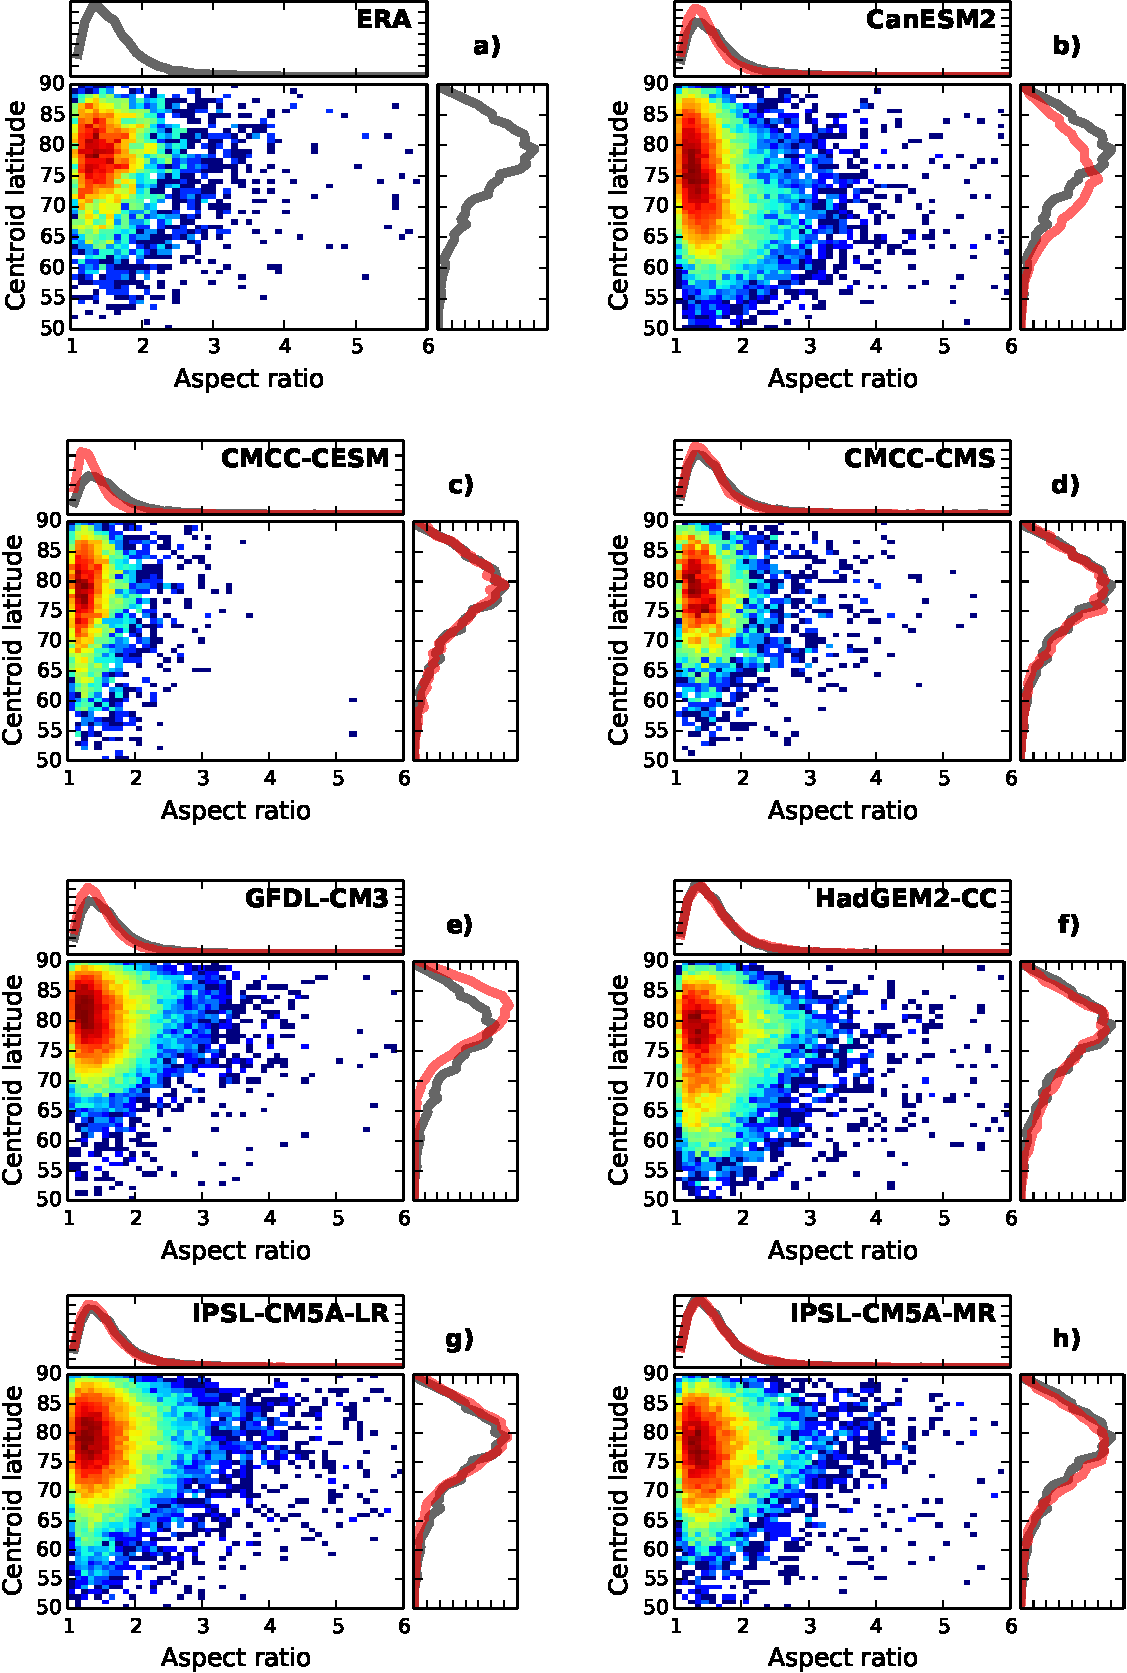
\includegraphics[width=\textwidth]{figures/chapter-models/moments_stats1.pdf}
 \caption[Distributions of moment diagnostics for the CMIP5
 models.]{Distributions of centroid latitude and aspect ratio for the ERA (grey
   lines) (a) and the CMIP5 models (red lines). Joint distributions are shown
   with a logarithmic scale such that red squares represent the densest
   regions.}
 \label{fig:cmip5_moments_stats}
\end{figure}

\begin{figure}[htbp]
 \ContinuedFloat
 \centering
 \noindent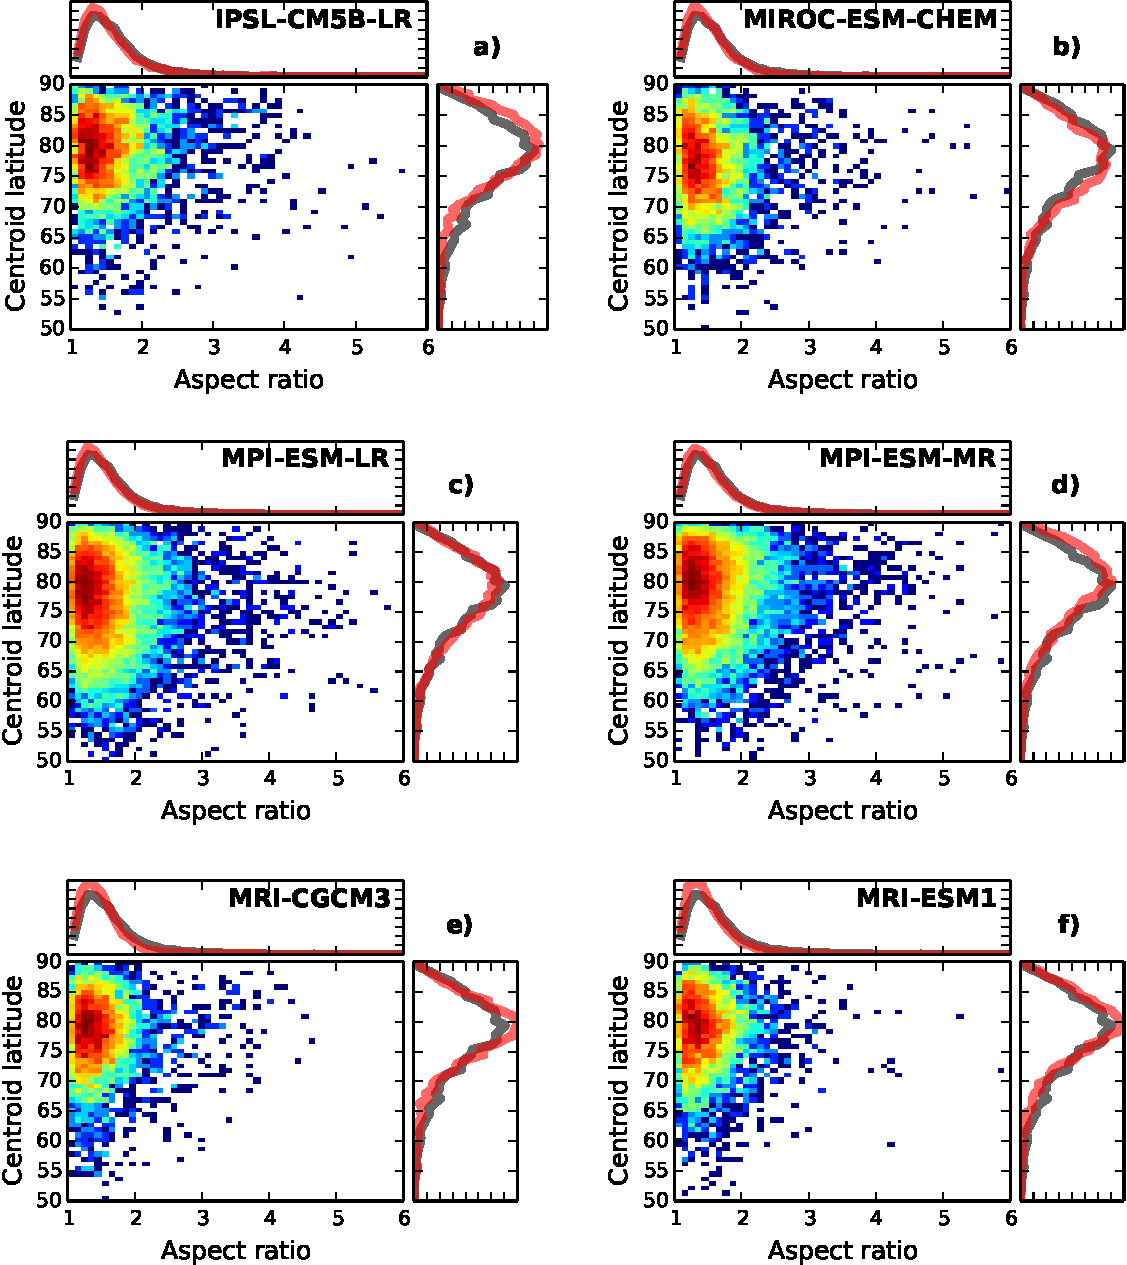
\includegraphics[width=\textwidth]{figures/chapter-models/moments_stats2.pdf}
 \caption[]{(Continued)}
\end{figure}


The centroid latitude and aspect ratio moment diagnostics are calculated for
each of the CMIP5 models over DJFM from the 10~hPa geopotential height field,
using the method described in Section \ref{sec:vort-geom-calc}. For each model
the value of the DJFM mean geopotential height at 60$^{\circ}$N and 10~hPa is
used to define the appropriate contour for the calculation of the moment
diagnostics. This accounts for biases in the mean geopotential height between
different models.

The resulting joint distributions of daily centroid latitude and aspect ratio
from each of the models are shown in Figure \ref{fig:cmip5_moments_stats}, along
with that from the ERA-40/ERA-Interim reanalysis (hereafter ERA) calculated in
Chapter \ref{cha:moments}. For each model the joint distribution histogram is
plotted with a logarithmic colour scale which is normalised according to the
number of days entering each box. As discussed in Chapter \ref{cha:moments}, it
can be seen that the joint distribution for ERA has an approximately triangular
distribution with high aspect ratio/poleward centroid latitude, and low aspect
ratio/equatorward centroid latitude being relatively more common than
high aspect ratio/equatorward centroid latitude. This shape of distribution is
well replicated by most of the models, although CanESM2 has a significantly
different shape, with the high aspect ratio/equatorward centroid latitude being
more common. 

No clear consistent biases among models emerge from this analysis. CanESM2 has a
modal centroid latitude which is about $5^{\circ}$ too far equatorward compared
to reanalysis. Contrastingly, GFDL-CM3 has a modal centroid latitude about
$2.5^{\circ}$ more poleward than observed. CMCC-CESM displays a clear bias in
the aspect ratio, with a distribution much less skewed towards high values than
in reanalysis.

The winter seasonal cycle of aspect ratio and centroid a latitude in the CMIP5
models is shown in Figure \ref{fig:cmip5_moments_stats_seas}. For the mean
aspect ratio and centroid latitude, the majority of models agree well with
reanalysis. CMCC-CESM has a consistently too low mean aspect ratio, while
GFDL-CM3 has a consistently too poleward mean centroid latitude, indicating that
these biases are not strongly seasonally dependent. On the other hand, the large
equatorward bias in the CanESM2 mean centroid latitude is much larger in
December and early January than later in winter. The 95th percentile of aspect
ratio is lower than reanalysis for the majority of models throughout the season,
indicating that models have, on average, too little variability in aspect ratio
 
\begin{figure}
 \centering
 \noindent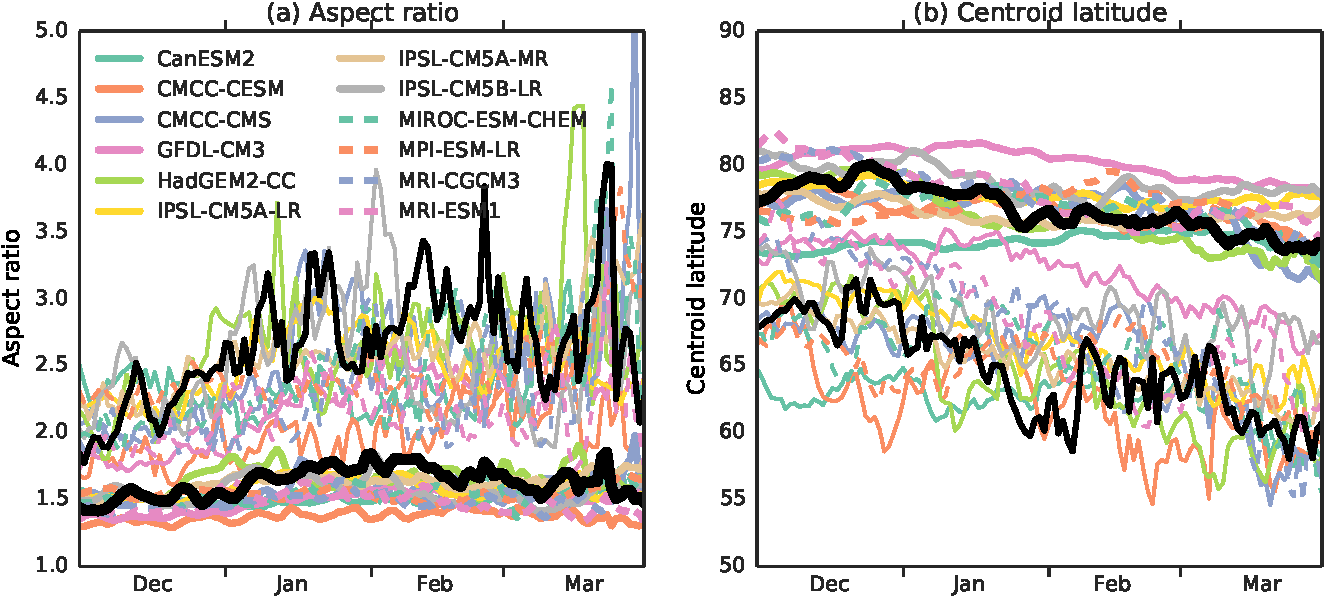
\includegraphics[width=\textwidth]{figures/chapter-models/moments_seasonal_stats.pdf}
 \caption[Seasonal cycle of moment diagnostics in the CMIP5 models]{Seasonal
   cycle of aspect ratio and centroid latitude in ERA (black) and the CMIP5
   models (colours). Thick lines represent the mean and thin lines the 95th or
   5th percentile for aspect ratio and centroid latitude respectively.}
 \label{fig:cmip5_moments_stats_seas}
\end{figure}


\subsection{Displaced and split vortex events}

Displaced and split vortex events are identified within the CMIP5 ensemble using
the threshold-based method described in Section \ref{sec:event-definition}. The
same thresholds as used for ERA (66$^{\circ}$N for centroid latitude and 2.4 for
aspect ratio) are used for the models in order to identify, as much as possible,
geometrically equivalent events. The same persistence of 7 days was also used.
The frequency of displaced and split vortex events for each model is shown in
Figure \ref{fig:cmip5_events_bar_stacked}.

\begin{figure}[htbp]
 \centering
 \noindent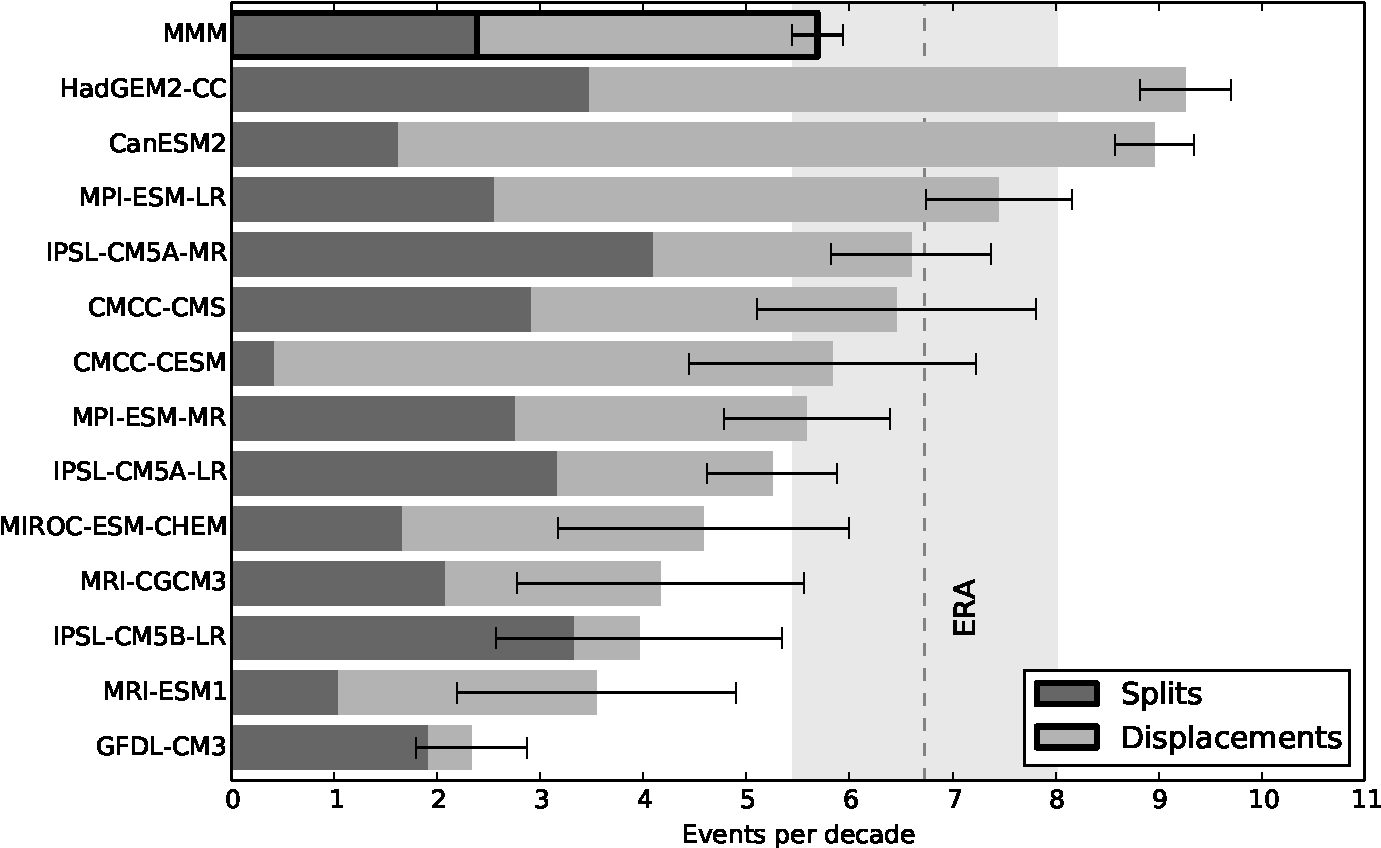
\includegraphics[width=\textwidth]{figures/chapter-models/events_bar_stacked.pdf}
 \caption[Frequency of split and displaced vortex events in the CMIP5
 models]{Frequency of split and displaced vortex events in the CMIP5 models,
   ERA, and the multi-model mean (MMM). Error bars are for the frequency of all
   events, and represent one $\sigma$ range, assuming a binomial distribution of
   events. The grey shaded region represents the one $\sigma$ range for ERA,
   along with the mean (dashed line.) }
 \label{fig:cmip5_events_bar_stacked}
\end{figure}

The total frequency of displaced and split vortex events for each of the CMIP5
models agrees well with the equivalent SSW frequency calculated by
\citet{Charlton-Perez2013}, who identified events based on the reversal of
zonal-mean zonal wind at 60$^{\circ}$N and 10~hPa. They also found HadGEM2-CC to
have the highest frequency of events within the CMIP5 ensemble, while MRI-CGCM3
is the model with the lowest frequency of SSWs in their study (excluding GFDL-CM3
and MRI-ESM1 which \citet{Charlton-Perez2013} did not analyse, MRI-CGCM3 is the
second-lowest frequency in the present study). This similarity between
\citet{Charlton-Perez2013} and the present study indicates that the close
relationship between moment diagnostics-defined events and SSWs defined by
zonal-mean zonal wind, as described in Chapter \ref{cha:moments}, also holds for
climate models (although this is not explicitly studied here).

As well as the large differences in the total frequency of displaced and split
vortex events, it can be seen in Figure \ref{fig:cmip5_events_bar_stacked} that
the ratio of frequencies of these events varies significantly between
models. For instance CanESM2 and CMCC-CESM simulate almost entirely displaced
vortex events, while IPSL-CM5B-LR and GFDL-CM3 simulate almost entirely split
vortex events. In the multi-model mean (MMM) these biases largely cancel, to
give a approximately equal ratio of displaced to split vortex events, which is
in agreement with reanalysis.

The seasonal distribution of these displaced and split vortex events is
illustrated in Figure \ref{fig:cmip5_events_seasonal}. Some models (CMCC-CMS,
HadGEM2-CC and IPSL-CM5A-LR) replicate the observed distribution, with split
vortex events being more likely in early winter, and displaced vortex events in
late winter. Other models, however, have a very different
distribution of events. CanESM2, CMCC-CESM and MPI-ESM-LR all show little
seasonal variability in the frequency of events. 


\begin{figure}
 \centering
 \noindent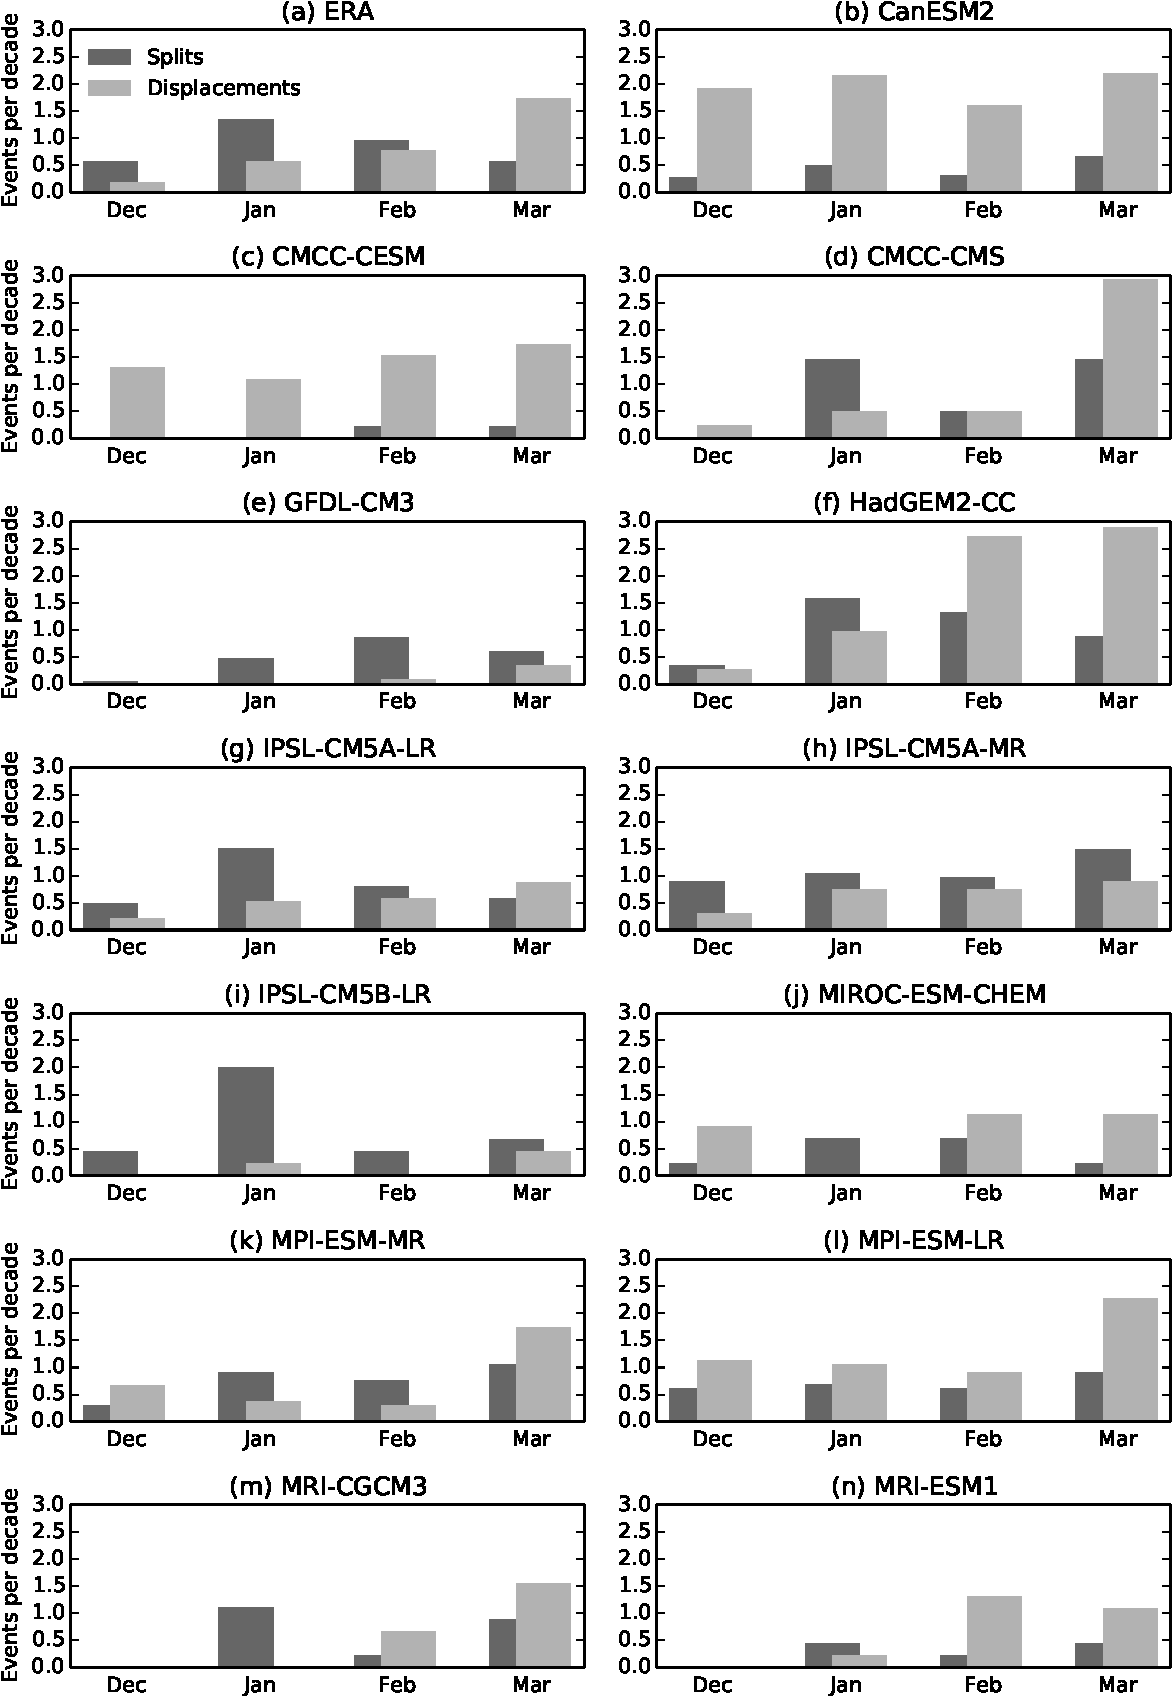
\includegraphics[width=\textwidth]{figures/chapter-models/events_seasonal.pdf}
 \caption[Seasonal distribution of splits and displacements in the CMIP5
 models]{Seasonal distribution of the occurrence of split and displaced vortex
   events in ERA (a) and the CMIP5 models.}
 \label{fig:cmip5_events_seasonal}
\end{figure}

\bigskip It is now considered how model biases in the climatology of the
stratospheric polar vortex, discussed in Section \ref{sec:moment-diagnostics},
affect the frequency of split and displaced vortex events. The climatological
average state of the vortex is defined by the mode -- the peak of the
probability distribution function -- of the aspect ratio and centroid
latitude. Unlike the mean, this quantity is not affected by extreme values and
it represents the average undisturbed state of the vortex. The peak can be
estimated by the maximum value of a histogram, however this introduces
significant random errors and is sensitive to the selection of bin size. A more
accurate estimation of the mode can be made by fitting the aspect ratio and
centroid latitude with a theoretical distribution and then finding the peak of
that distribution. Following \citet{Mitchell2011}, we fit the aspect ratio with
a generalised extreme value (GEV) distribution of the form
\begin{equation}
f(x;\mu,\sigma,\xi) = \frac{a^{(-1/\xi)-1}}{\sigma}\mathrm{e}^{{-a}^{-1/\xi}}
\quad , 
\end{equation}
with
\begin{equation} 
a = 1 + \xi \frac{x-\mu}{\sigma} \quad ,
\end{equation}
where $\mu$ determines the position of the peak along the $x$-axis, $\sigma$
determines the variance of the distribution and $\xi$ the skewness. These
parameters are determined using the method of maximum-likelihood estimation
\citep{Wilks}. This method is also used to fit a Gaussian distribution of the
form
\begin{equation}
f(x;\mu,\sigma) = \frac{1}{\sigma\sqrt{2\pi}} \left(
  -\frac{(x-\mu)^2}{2\sigma^{2}} \right) \quad ,
\end{equation}
where $\mu$ determines the position of the peak along the $x$-axis and $\sigma$
is the standard deviation, to the cube of the centroid latitude, and then the
cube root taken to return the original distribution. \citet{Mitchell2011} found
that these distributions accurately fit the histograms of centroid latitude and
aspect ratio in reanalysis data, apart from the extreme tails of the
distribution. Qualitative inspection of the distribution for each model confirms
that they also provide a similarly good fit to each of the model's histograms.

Figure \ref{fig:cmip5_moments_scatter} shows the relationship between the modal
aspect ratio and centroid latitude and frequency of split and displaced vortex
events. It can be seen that strong linear relationships exist; the modal aspect
ratio accounts for 79\% of the variance in the frequency of split vortex events
and the modal centroid latitude accounts for 76\% of the variance in the
frequency of displaced vortex events. This demonstrates that biases in the
average undisturbed state of the vortex account for the vast majority of
inter-model spread in the representation of extremes. An implication of this is
that the models are consistent in their representation of the variability of
aspect ratio and centroid latitude, relative to the model climatology.

It can also be seen in Figure \ref{fig:cmip5_moments_scatter} that the values
for ERA lie very close to the best fit lines of the CMIP5 models. This implies
that the accuracy of a model's representation of the frequency of displaced and
split vortex events can be significantly improved by a more accurate average
undisturbed vortex state. Furthermore, while the ERA value for modal centroid
latitude lies approximately in the middle of that for the CMIP5 models, only two
models have a larger modal aspect ratio than ERA, indicating that a too
circularly-symmetric vortex is a common bias among models.

\begin{figure}
 \centering
 \noindent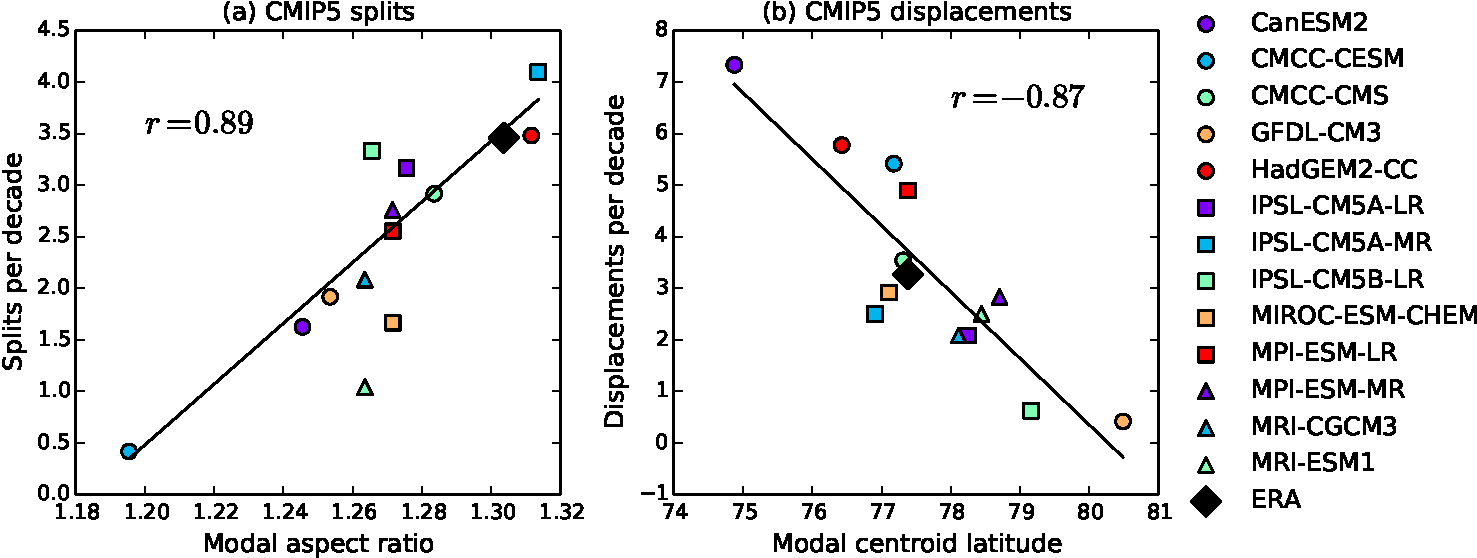
\includegraphics[width=\textwidth]{figures/chapter-models/CMIP5_moments_scatter.pdf}
 \caption[Comparison of moment diagnostics and frequency of split and displaced
 vortex events.]{Comparison of the DJFM mean aspect ratio with frequency of
   split vortex events (a) and DJFM mean centroid latitude with frequency of
   displaced vortex events (b) in the CMIP5 ensemble and ERA. Linear best fits
   and the correlation coefficients for all the models are also shown.}
 \label{fig:cmip5_moments_scatter}
\end{figure}

The structure of the stratospheric polar vortex during split and displaced
vortex events in the CMIP5 ensemble is shown in Figure
\ref{fig:10hPa_GPH_comp}. This displays composites of 10~hPa geopotential height
at the onset date of the events for each model. It can be seen that the majority
of models accurately reproduce splitting events as occurring along the
$90^{\circ}$W-$90^{\circ}$E axis, and displacement events with a vortex shifted
towards Scandinavia and Siberia. CanESM2 is an exception to this, with split
vortex events which are elliptical but centred quite far from the pole. The
IPSL-CM5B-LR model also has a very different appearance of displaced vortex
events, although this composite only consists of three events so differences are
unlikely to be statistically significant. There is also significant inter-model
spread in the relative strengths of the Aleutian and Azores highs during split
vortex events. Several models (GFDL-CM3, IPSL-CM5A-LR, IPSL-CM5B-LR, MRI-ESM1)
show an approximately equal strength Aleutian and Azores highs, while others
(CMCC-CMS, HadGEM2-CC, IPSL-CM5A-MR, MPI-ESM-LR, MPI-ESM-MR, MRI-CGCM2) show a
weaker Azores high, which is in closer agreement with reanalysis. The more
symmetrical Aleutian and Azores highs indicate a greater dominance of wave-2
activity in split vortex events than is found in observations, where not all
split vortex events are dominated by wave-2 activity
\citep{Waugh1997,Mitchell2013}.

\begin{figure}
 \centering
 \noindent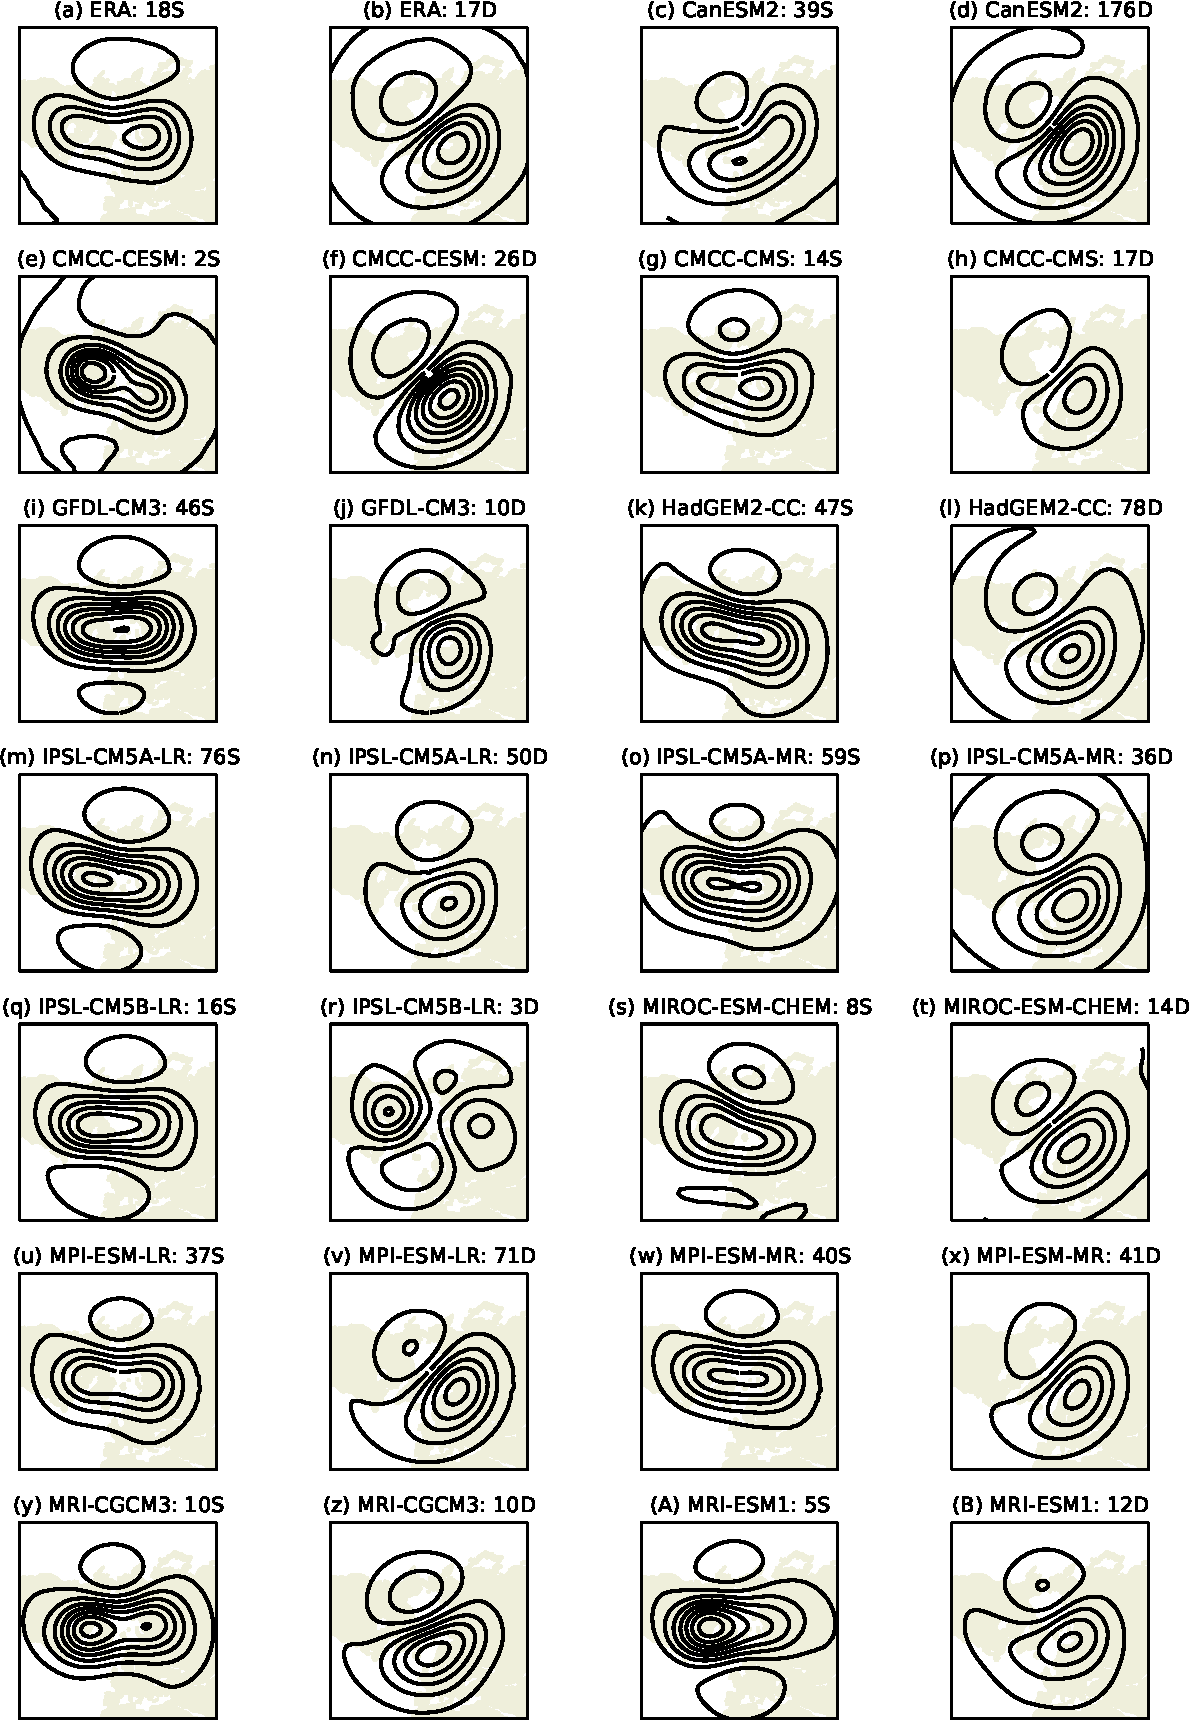
\includegraphics[width=\textwidth]{figures/chapter-models/10hPa_GPH_composites.pdf}
 \caption[Composites of 10~hPa $Z$ at the onset date split and displaced vortex
 events in the CMIP5 models.]{Composites of 10~hPa $Z$ at the onset date of
   split (S) and displaced (D) vortex events in ERA (a,b) and the CMIP5
   models. The number of events entering the composite and their type are
   shown in the title of each plot. The contour interval is 0.3~km.}
 \label{fig:10hPa_GPH_comp}
\end{figure}




\section{Stratosphere-troposphere coupling}
\subsection{Zonal-mean response to displaced and split vortex events}

The time-height evolution of the atmosphere around split and displaced vortex
events in each of the CMIP5 models is displayed in Figure
\ref{fig:cmip5_dripping_paint}. This shows composites of polar cap
($60^{\circ}$-$90^{\circ}$N) geopotential height ($Z$) anomalies from 90 days
before to 90 days following events. The anomalies are calculated from the
climatology of each day for each model. The figures extend downwards only to
500~hPa (rather than 1000~hPa). This is because models differ in their
representation of geopotential height which is below ground level; some allow
negative values, while others set this as an undefined value. This introduces
significant errors in the calculation of a climatology and anomalies at levels
where the geopotential height is occasionally below ground level. Polar cap $Z$
is highly correlated with the NAM (calculated from zonal mean $Z$ according to
the method of \citet{Baldwin2009}) over the levels shown in Figure
\ref{fig:cmip5_dripping_paint}. \citet{Kushner2010} also demonstrated composites
of the NAM and polar cap $Z$ following SSWs to be very similar. Indeed,
comparing Figures \ref{fig:cmip5_dripping_paint} (a) and (b) with Figure
\ref{fig:dripping_paint} shows that the ERA composites for polar cap $Z$ and the
NAM are very similar. In Figure \ref{fig:cmip5_dripping_paint} the number of
events entering each composite is shown in the upper right-hand corner, and it
should be noted that composites of a small number of events are likely to be
subject to significant statistical uncertainty.

It can be seen that there are large inter-model differences in the evolution of
polar cap $Z$ following split and displaced vortex events. For some models
(e.g. CanESM2, CMCC-CMS) lower stratospheric anomalies persist for about 45
days, similar to reanalysis, while for others (e.g. IPSL-CM5A-LR, GFDL-CM3)
these persist for much longer, beyond 60 days. There are also differences in the
stratospheric precursors to events; while some models (e.g. CanESM2, GFDL-CM3,
MRI-CGCM3) simulate a stronger negative anomaly prior to displacement events,
similar to reanalysis, others (HadGEM2-CC, IPSL-CM5A-MR, MRI-ESM1), show more
negative anomalies prior to split vortex events. 

Most significantly, there is a large spread in the tropospheric anomalies over
the 10-90 days following split and displaced vortex events. Several models
(e.g. IPSL-CM5A-LR, IPSL-CM5A-MR, MPI-ESM-LR) show only very weak anomalies
below approximately 200~hPa, while others (e.g., CMCC-CESM, GFDL-CM3, MRI-ESM1)
show stronger anomalies. Among those models which do show stronger tropospheric
anomalies, there are also differences in the relative magnitude following split
and displaced vortex events. For instance, for GFDL-CM3, and MRI-ESM1
tropospheric anomalies following displaced vortex events are stronger, while for
MIROC-ESM-CHEM and MPI-ESM-MR anomalies following split vortex events are
stronger, in closer agreement with reanalysis. 

As well as these large inter-model differences, there are also some consistent
features among models. Almost all models show a barotropic onset to split vortex
events, with anomalies occurring at the same time throughout the depth of the
atmosphere. In contrast, displaced vortex events apprear more baroclinic, with
onset occurring first near the uppermost level. This is consistent with the
difference found in reanalysis, indicating that this is likley to be a robust
difference between the response to split and displaced vortex events. These
features are also apparent in the multi-model mean (MMM) (Figures
\ref{fig:cmip5_dripping_paint} C and D). This mean is calculated so as to give
each event an equal weight (rather than each model), and so does not give undue
weight to models with only a small number of events. On the other hand this does
mean that greater weight is given to models with more ensemble members and more
events (almost one third of all displaced vortex events come from CanESM2), but
the difference in baroclinicity of split and displaced vortex events is observed
to be very consistent among models.

\begin{figure}
 \centering
 \noindent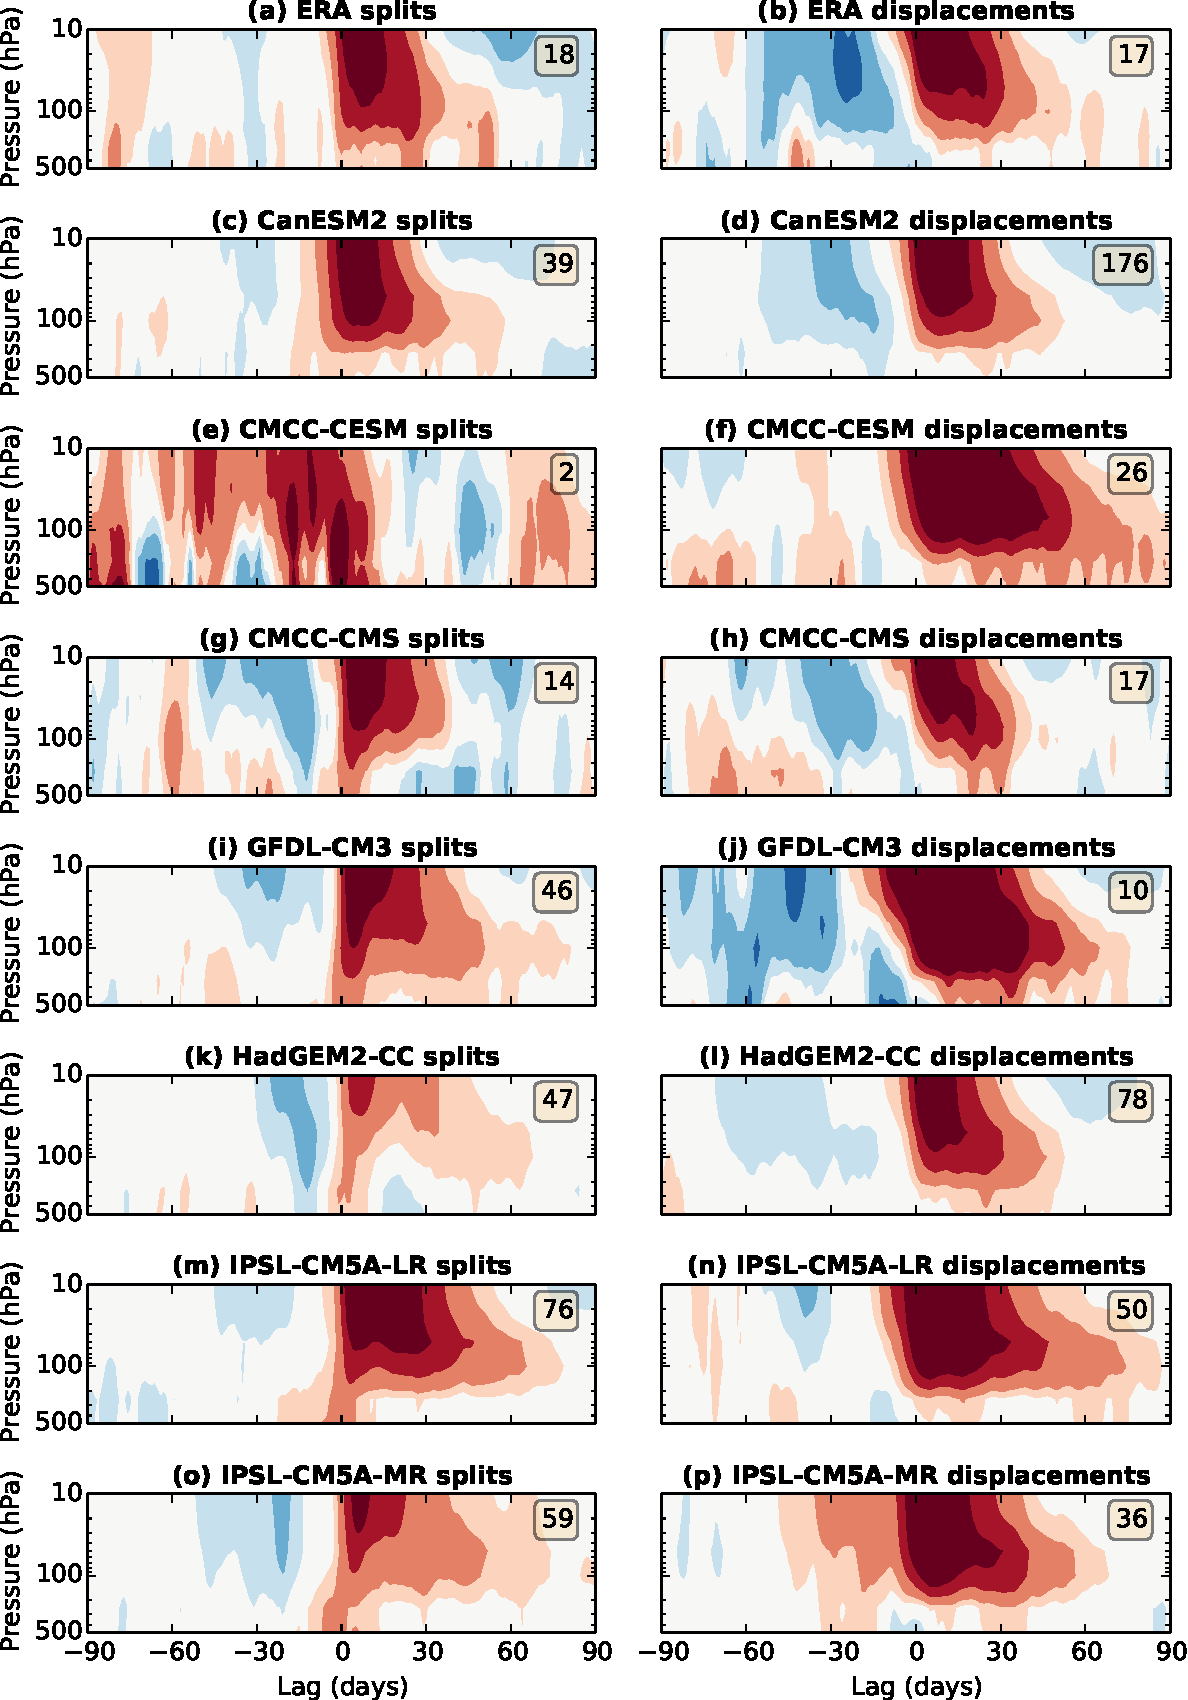
\includegraphics[width=\textwidth]{figures/chapter-models/dripping_paint1.pdf}
 \caption[NAM composites for splits and displacements in the CMIP5
 models]{Composites of normalised polar cap averaged $Z$ anomalies following
   split and displaced vortex events in ERA (a,b), the CMIP5 models, and the
   multi-model mean (C,D). Numbers in the upper right of each plot represent the
   number of events entering the composite.}
 \label{fig:cmip5_dripping_paint}
\end{figure}

\begin{figure}
 \ContinuedFloat
 \centering
 \noindent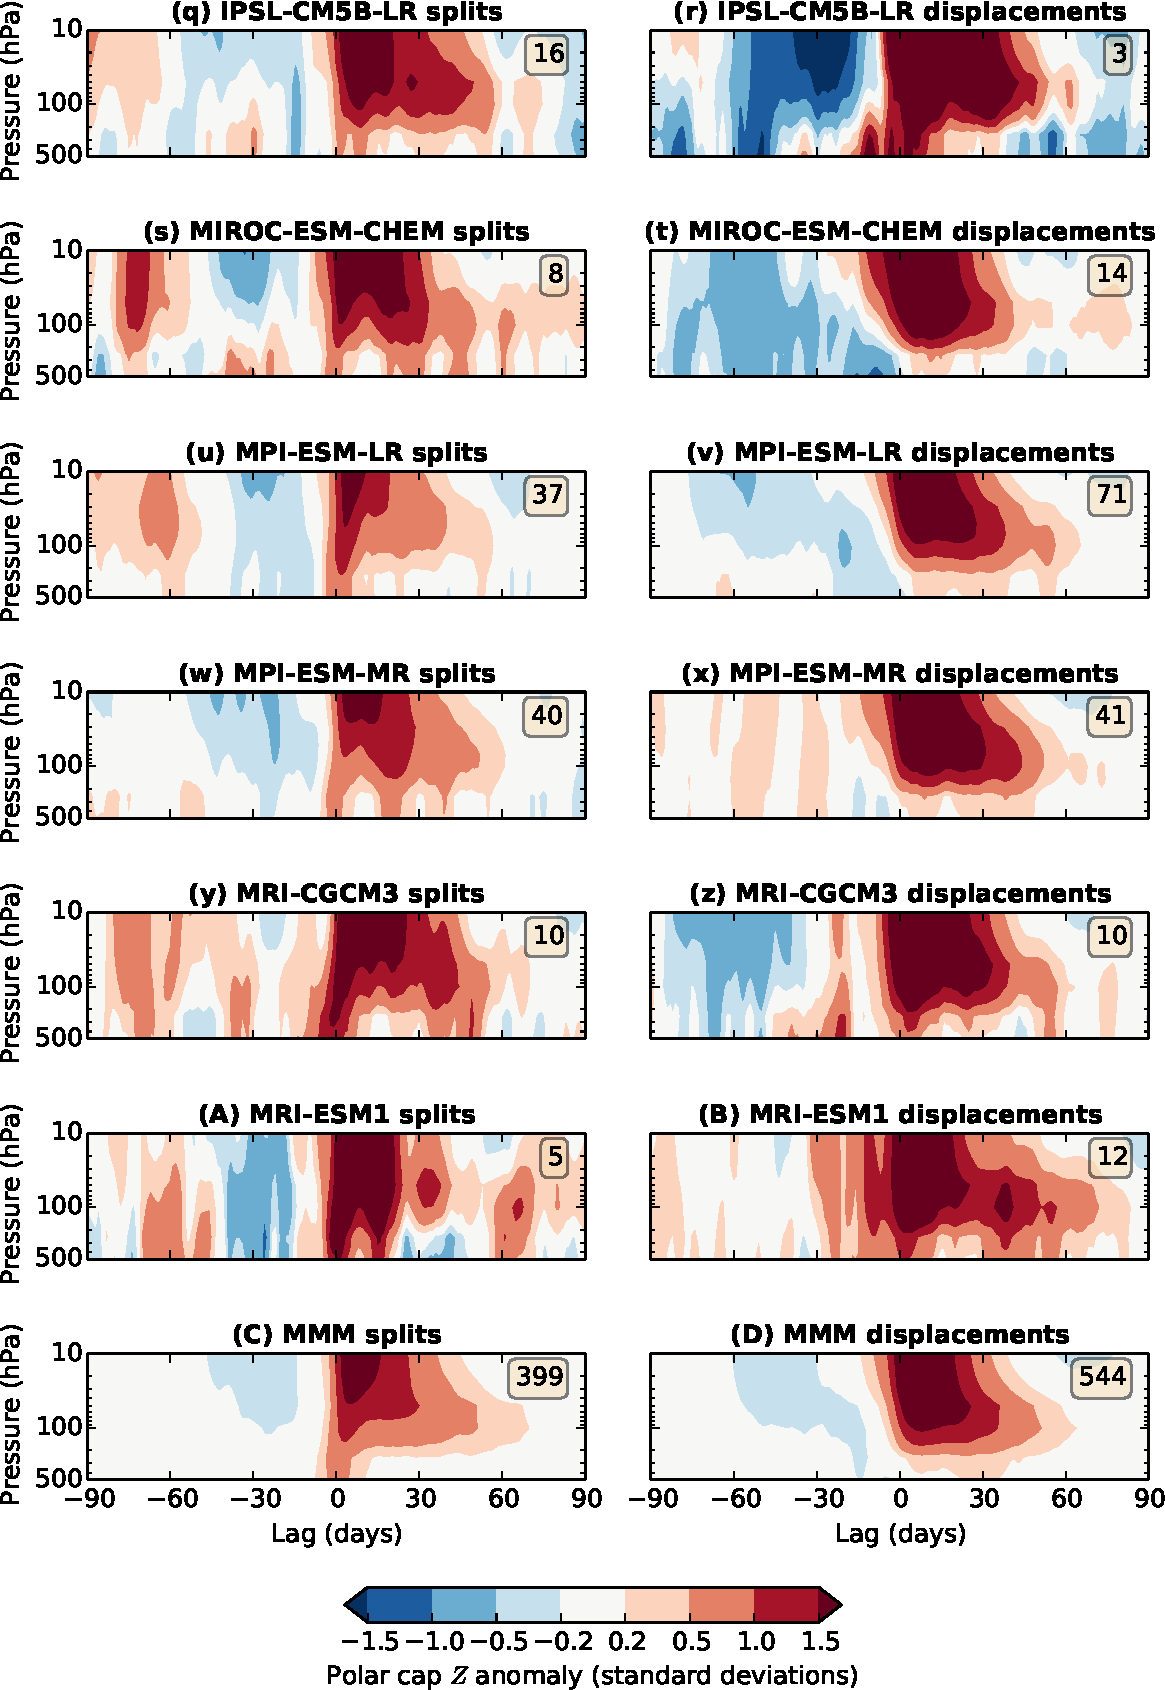
\includegraphics[width=\textwidth]{figures/chapter-models/dripping_paint2.pdf}
 \caption[]{(Continued)}
\end{figure}


\subsection{Spatial response to displaced and split vortex events}

\begin{figure}
 \centering
 \noindent\includegraphics[width=\textwidth]{figures/chapter-models/mslp_composites.pdf}
 \caption[MSLP composites following splits and displacements in the CMIP5
 models]{Composites of mean sea-level pressure anomalies averaged 0-30 days
   following split (S) and displaced (D) vortex events in the CMIP5
   ensemble. Also shown are the ERA composite (a,b) and the multi-model mean
   (C,D). The multi-model mean is calculated as to give each event an equal
   weighting.}
 \label{fig:cmip5_mslp_comp}
\end{figure}

\begin{figure}
 \centering
 \noindent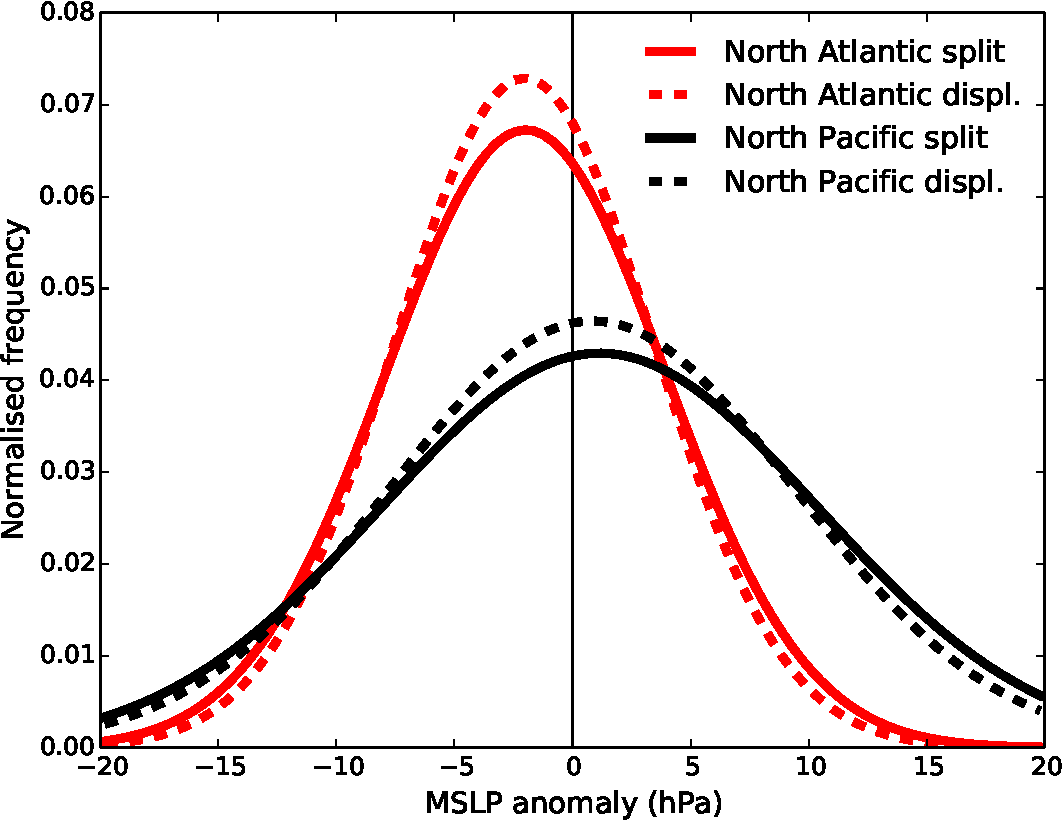
\includegraphics[width=0.7\textwidth]{figures/chapter-models/NAO_PNA_histogram.pdf}
 \caption[Distribution of MSLP anomalies in North Pacific and Atlantic following
 splits and displacements.]{Distribution of mean sea-level pressure anomalies in
   the central North Atlantic ($38^{\circ}$N, $26^{\circ}$W) and central North
   Pacific ($45^{\circ}$N, $165^{\circ}$W) averaged over the 30 days following
   split and displacement events in all the CMIP5 models. These two locations
   correspond to centres of action of the NAO and PNA patterns
   respectively. Data are fitted with a Gaussian distribution.}
 \label{fig:cmip5_nao_pna}
\end{figure}

Mean sea-level pressure (MSLP) anomalies averaged over the 30 days following
split and displaced vortex events for each of the CMIP5 models are displayed in
Figure \ref{fig:cmip5_mslp_comp}. Also shown are the anomalies for ERA (a,b)
(the same as Figure \ref{fig:mslp_composites}) as well as the multi-model mean
(c,d), again calculated so as to give each event an equal weight. The
climatology from which anomalies are calculated is determined by a 10-day
running mean of the average for each day of the year at each spatial
location. The number of events entering each composite is shown, and again, care
must be taken interpreting composites of a small number of events due to
statistical uncertainty.

Following both split and displaced vortex events, all models show a positive
MSLP anomaly near the North Pole, and a negative anomaly centred over Western
Europe and the North Atlantic. This pattern is consistent with a negative
projection onto the North Atlantic Oscillation. Less consistent among models are
anomalies over the North Pacific; many models (e.g. MRI-CGCM3, IPSL-CM5A-LR)
show positive anomalies, while MPI-ESM-LR a MPI-ESM-MR have negative anomalies
following both split and displaced vortex events. MIROC-ESM-CHEM has different
sign anomalies in the North Pacific following split (negative) and displaced
(positive) vortex events. In the multi-model mean, a weakly positive North
Pacific anomaly is seen.

Figure \ref{fig:cmip5_nao_pna} illustrates that this difference in consistency
of the Atlantic and Pacific MSLP anomalies also exists in the multi-model
ensemble of all events. It shows the distribution of MSLP anomalies averaged 30
days following all modelled split and displaced vortex events at the approximate
centres of action of the NAO (over the Azores at $38^{\circ}$N, $26^{\circ}$)
and the Pacific-North American (PNA) pattern (central North Pacific at
$45^{\circ}$N, $165^{\circ}$W). The North Atlantic distribution is centred
further from zero and has a lower variance than the North Pacific distribution
for both split and displaced vortex events. This is despite the fact that the
standard deviation in monthly winter MSLP is approximately equal in the two
regions \citep{Allan2006}, and so again indicates the more consistent North
Atlantic response.

This inconsistency in the Pacific anomalies has important consequences for the
interpretation of zonal mean anomalies following split and displaced vortex
events. For instance, the IPSL-CM5A-LR model shows weak tropospheric anomalies
(relative to other models) of polar cap averaged $Z$ following split and
displaced vortex events (Figure \ref{fig:cmip5_dripping_paint} (m,n)), but a
relatively strong NAO signal (Figure \ref{fig:cmip5_mslp_comp} (m,n)),
particularly following split vortex events. The reason for this difference is
that the model also shows relatively strong positive North Pacific anomalies,
that to some extent cancel the North Atlantic anomalies in the polar cap
average. Such an effect would also be seen in the NAM, even if calculated from
non zonally-averaged $Z$, since the surface NAM pattern (the leading EOF of
MSLP) has centres of action of the same sign in the North Atlantic and North
Pacific \citep[e.g.,][]{Ambaum2001}.

A robust difference found between MSLP anomalies following split and displaced
vortex events in almost all models and the multi-model mean is that anomalies
over Russia and Eastern Europe are more strongly negative following displaced
vortex events. In the multi-model mean, this difference has a magnitude of about
2-3~hPa across most of Russia. In order to understand the possible stratospheric
influence on this difference, lower stratospheric anomalies are studied. Figure
\ref{fig:cmip5_100hPa_comp} shows composites of 100~hPa $Z$ averaged over the 10
days following the onset of split and displaced vortex events. This shorter time
period (rather than the 30 days used for the MSLP composites) is chosen to
represent the typical time scale of a split or displacement of the vortex, which
is shorter than the time scale taken for the re-formation of the vortex and
return towards the climatological mean. However, it should be noted that
composites taken over the 30 days show similar structure, but with reduced
magnitude (not shown). 

As well as the composite for each model, and the split minus displaced vortex
difference, a multi-model mean is also shown in Figure
\ref{fig:cmip5_100hPa_comp} (Q,R,S). Because this is a mean of model absolute
values, and models have different climatologies, the MMMs for split and
displaced vortices are scaled to have the same hemispheric mean magnitude. This
avoids introducing a bias in the climatology of any particular model into the
MMM difference. 

For all models with the exception of CanESM2, the 100~hPa $Z$ split vortex
composite shows an elliptical vortex with the major axis aligned along the
$90^{\circ}$W-$90^{\circ}$E line which is similar to the composite at 10~hPa
(Figure \ref{fig:10hPa_GPH_comp}). For the displaced vortex composite the
100~hPa vortex is centred over Siberia for almost all models, eastward of the
10~hPa composite which is centred over Scandinavia. This again highlights the
more barotropic nature of split vortex events compared to baroclinic displaced
vortex events, in which the vortex shows a westward tilt with height (as also
demonstrated by \citet{Matthewman2009}).

In the split minus displaced vortex difference, the majority of models show a
large positive region over Russia and Eastern Europe and a negative region
centred over northern Canada. The positive region over Siberia has a minimum,
which is negative in some cases, located near $90^{\circ}$E, which is consistent
with the position of minimum in the split vortex composite. It can be seen that
the multi-model mean difference (Figure \ref{fig:cmip5_100hPa_comp} (S)) is
remarkably similar to the reanalysis difference (Figure
\ref{fig:cmip5_100hPa_comp}), both in terms of the location and magnitude of
anomalies. This suggests that the CMIP5 models, on average, realistically
represent the evolution of split and displaced vortex events through the depth
of the stratosphere. Again, this result is consistent among the majority of
models, and so not highly sensitive to the exclusion or inclusion of any
particular model. 

\begin{figure}
 \centering
 \noindent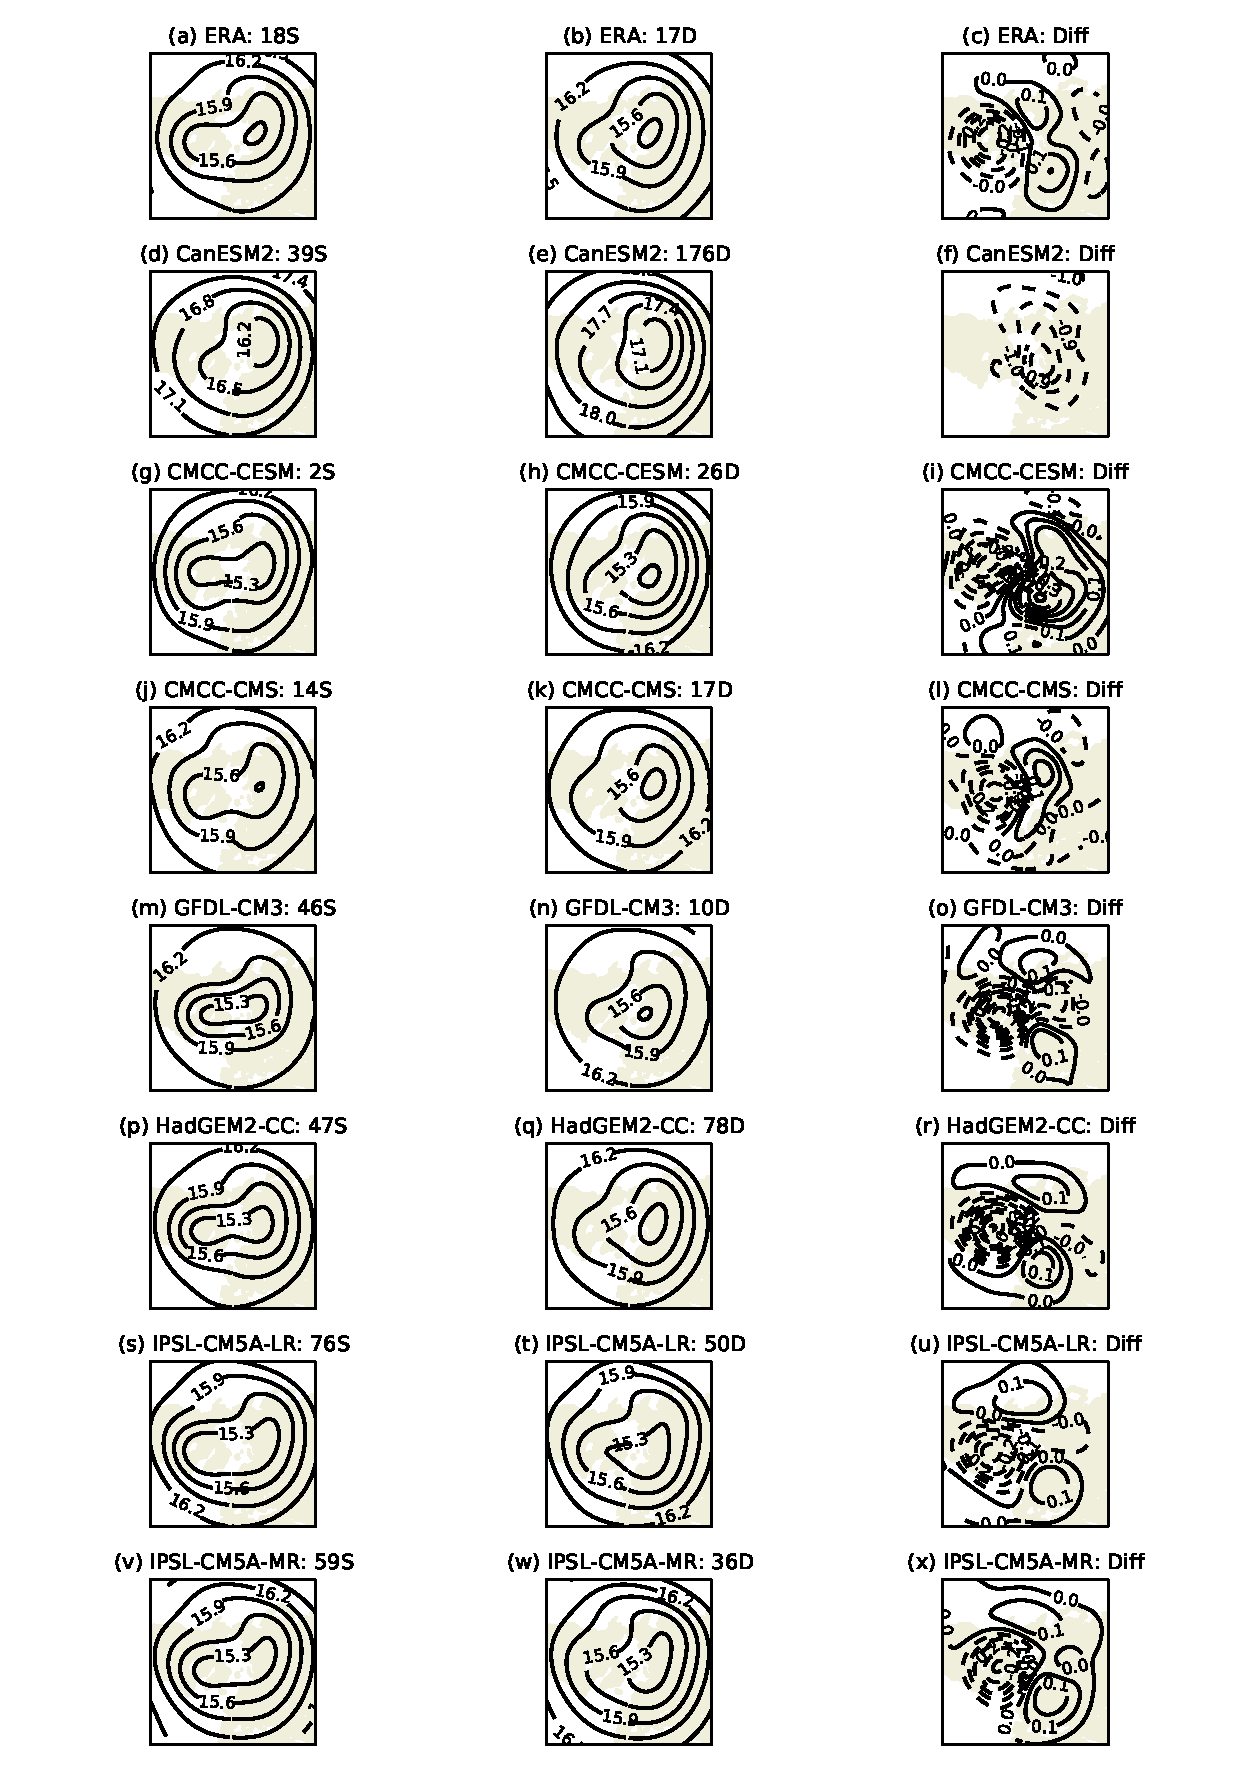
\includegraphics[width=\textwidth]{figures/chapter-models/100hPa_GPH1.pdf}
 \caption[NAM composites for splits and displacements in the CMIP5
 models]{Composites of 100~hPa geopotential height (km) averaged in the 10 days
   following the onset of split (S) and displaced (D) vortex events in ERA, each
   of the CMIP5 models, and the multi-model mean (MMM). The right hand column
   displays the difference of splits minus displacements. The multi-model mean
   is calculated so as to give each event an equal weighting.}
 \label{fig:cmip5_100hPa_comp}
\end{figure}

\begin{figure}
 \ContinuedFloat
 \centering
 \noindent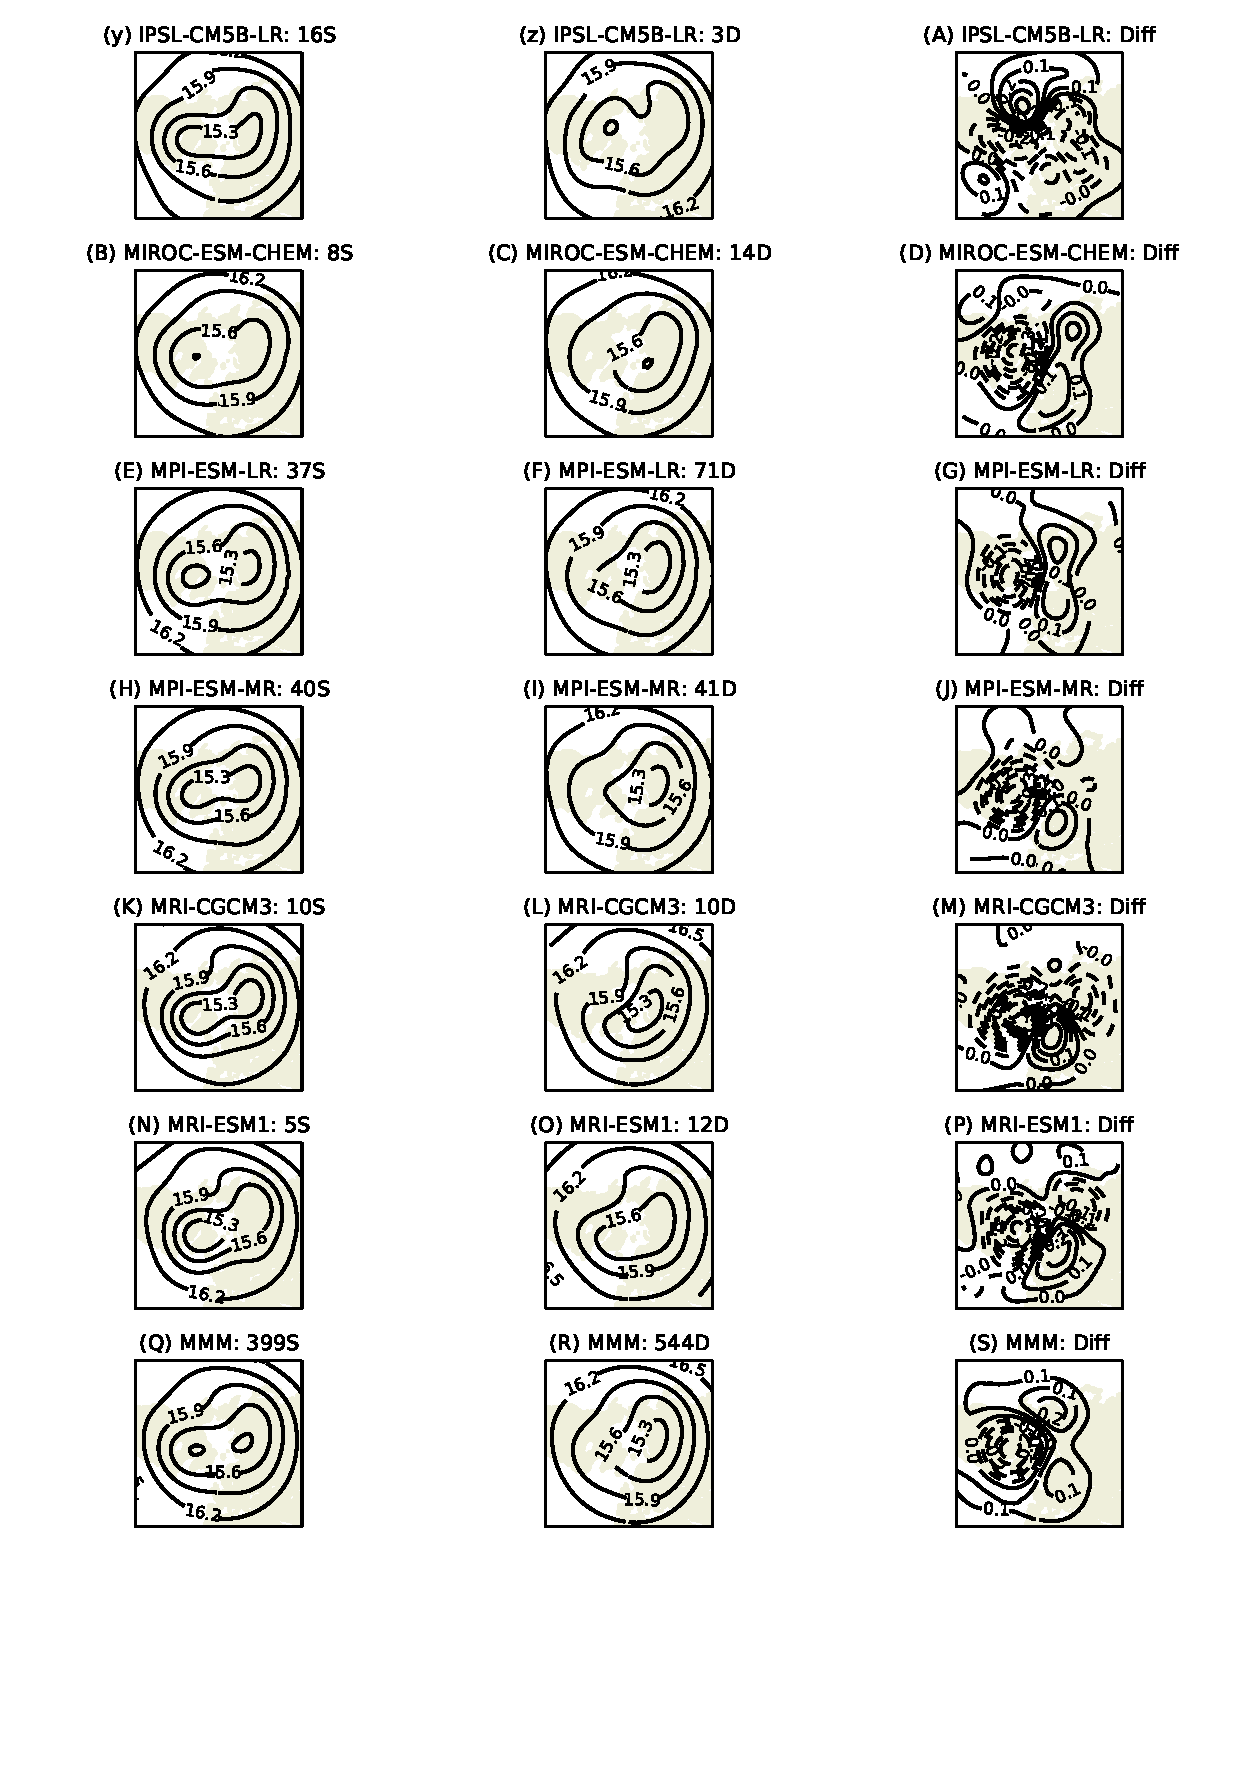
\includegraphics[width=\textwidth]{figures/chapter-models/100hPa_GPH2.pdf}
 \caption[]{(Continued)}
\end{figure}


\bigskip Figure \ref{fig:cmip5_mslp_diff} shows the split minus displaced vortex
composite difference for MSLP averaged 0-30 days following onset and the 100~hPa
$Z$ composite difference averaged 0-10 days following onset, for both ERA and
the CMIP5 MMM. Statistical significance in the MSLP difference is calculated by
a two-tailed bootstrap test with the null hypothesis that the anomalies
following split and displaced vortex events are populations from the same
probability distribution. The following procedure is used:
\begin{enumerate}
\item All events are grouped together and selected from them, with replacement,
  are two random subsets which are equal in size to the total number of split
  and displaced vortex events respectively.
\item The difference of the averages of these two subsets is taken.
\item The above is repeated 5000 times to form a distribution of random
  composite differences.
\item If the actual composite difference lies lower than the 2.5\% or higher
  than the 97.5\% levels of this distribution then it can be said there is a
  less than 95\% chance that an anomaly at least this large would arise if
  anomalies following split and displaced vortex events are populations from the
  same distribution. Hence the null hypothesis can be rejected.
\end{enumerate}
For the case of ERA, very little statistical significance in the
composite difference is seen, while in the CMIP5 MMM there are large
statistically significant regions. This is due to the greatly increased sample
size in CMIP5; a total of 943 events compared to just 35 in ERA. 

In the CMIP5 MMM difference the largest feature is the large positive anomaly (a
result of a more negative anomaly following displaced vortex events) over
Scandinavia, Eastern Europe and Russia. There is also a significant negative
anomaly over northern Canada and a positive anomaly in the western
Atlantic. This pattern is zonally asymmetric and so does not project strongly
onto the polar cap average, therefore explaining the small difference in polar
cap averaged $Z$ (Figure \ref{fig:cmip5_dripping_paint} (C,D)). The CMIP5
difference pattern also does not strongly project onto the NAO as there is a
similarly negative NAO following both split and displaced vortex events (Figure
\ref{fig:cmip5_mslp_comp} (C,D)). For the ERA MSLP difference there are stronger
negative anomalies over Europe (although not statistically significant) and
positive anomalies over the North Pole, which does project more strongly onto
the NAO, as discussed in Section \ref{sec:moments_analysis}. 

The CMIP5 difference of Figure \ref{fig:cmip5_mslp_diff} shows the positive
100~hPa $Z$ anomalies over Siberia over-lie the positive MSLP anomalies, while
the negative 100~hPa $Z$ over northern Canada over-lies negative MSLP
anomalies. A somewhat similar, but not statistically significant pattern is seen
in ERA, although the Siberian anomaly is more polewards and the negative anomaly
over Canada is much weaker. Importantly, the 100~hPa pressure surface lies
close to the tropopause, and 100~hPa $Z$ can therefore give an indication of
tropopause height. Indeed, comparing the 100~hPa $Z$ and tropopause height
anomalies for ERA (Figures \ref{fig:cmip5_100hPa_comp} (a,b) and
\ref{fig:tropopause_height} (c,d)) shows that anomalous negative $Z$ is
approximately co-located with an anomalously high tropopause, although the
tropopause height field is much noisier. 



\begin{figure}
 \centering
 \noindent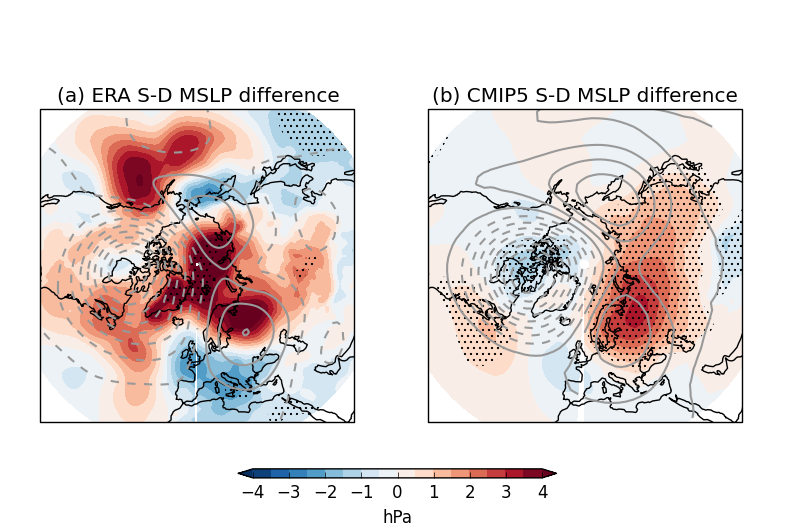
\includegraphics[width=\textwidth]{figures/chapter-models/mslp_diff.png}
 \caption[Difference of MSLP following split and displaced vortex
 events.]{Difference (S-D) of composites of mean sea-level pressure averaged
   0-30 days following split (S) and displaced (D) vortex events in ERA and the
   CMIP5 ensemble. Stippling indicates regions that are $>$95\% significant
   according to a two-tailed bootstrap test. Grey contours represent the
   difference in 100~hPa geopotential height averaged 0-10 days following events
   the contour interval is 40~m, dashed contours represent negative values and
   the lowest magnitude contours are $\pm$20~m. }
 \label{fig:cmip5_mslp_diff}
\end{figure}





\section{Discussion}
\subsection{Effect of model resolution}


\begin{figure}
 \centering
 \noindent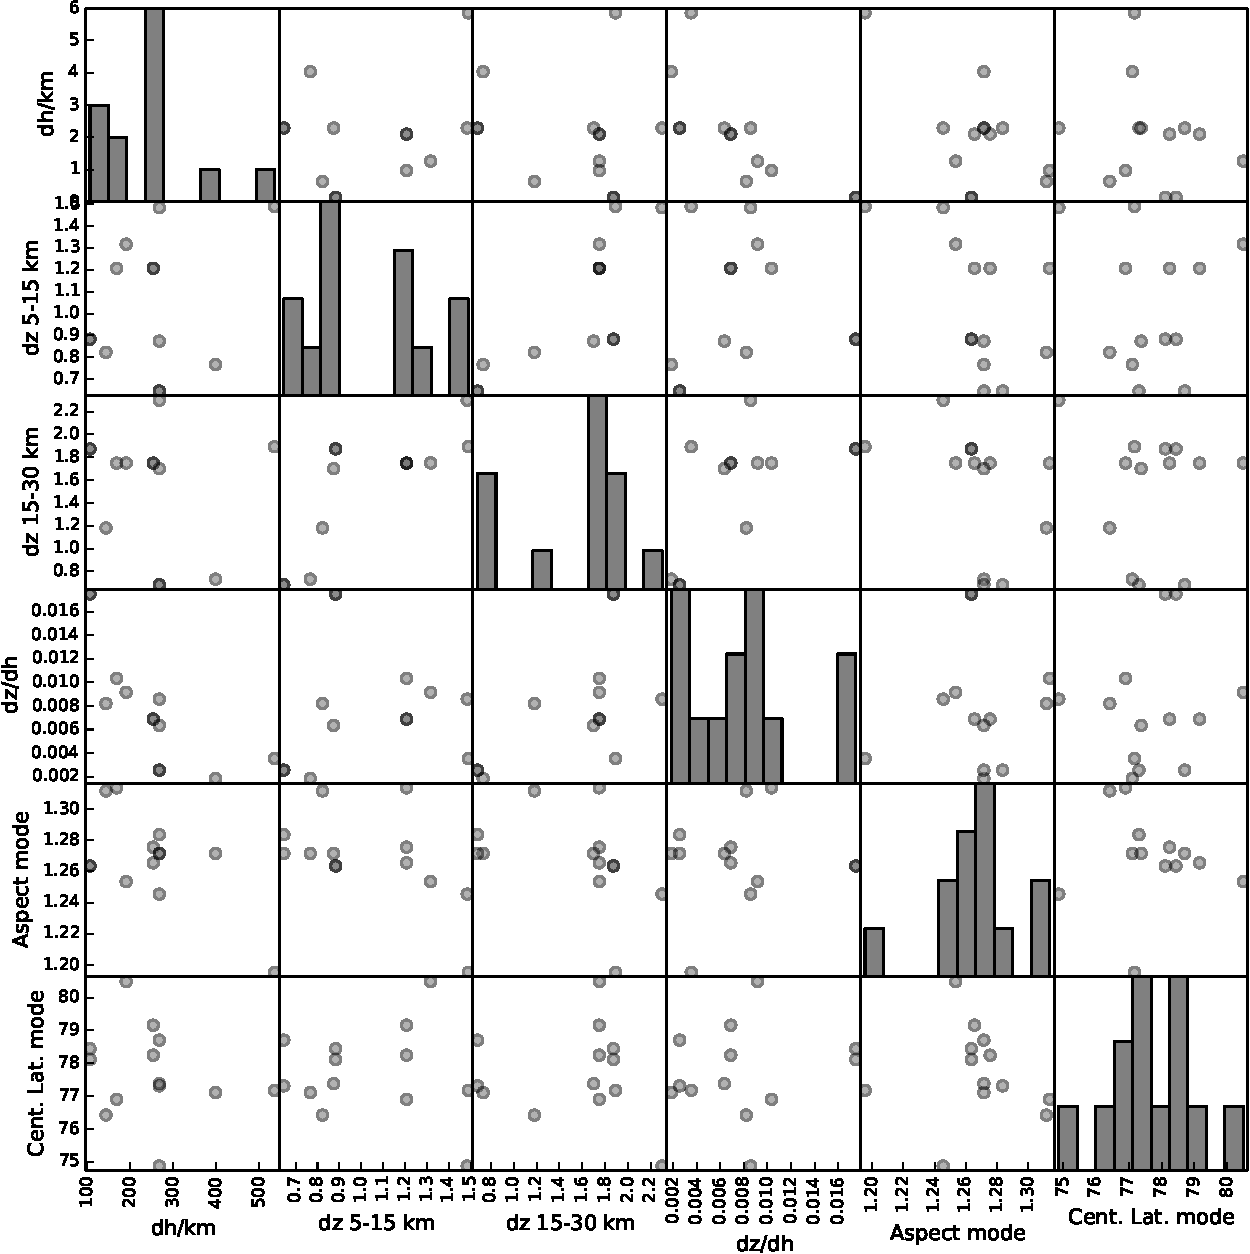
\includegraphics[width=\textwidth]{figures/chapter-models/scatter_matrix.pdf}
 \caption[Relationship between model resolution and moment diagnostics in the
 CMIP5 models.]{Relationship between model resolution, moment diagnostics, and
   stratosphere-troposphere coupling in the CMIP5 models. Model resolution is
   shown as horizontal resolution ($\mathrm{d}h$), vertical resolution
   ($\mathrm{d}z$) over 5-15~km and 15-30~km, and aspect ratio
   ($\mathrm{d}z$(5-15~km)$ / \mathrm{d}h$). Histograms for the relevant
   quantities are shown along the leading diagonal.}
 \label{fig:scatter_matrix}
\end{figure}

We have demonstrated that there are large differences in the representation of
the average undisturbed state of the stratospheric polar vortex among high-top
CMIP5 models. This amounts to an inter-model range in the modal centroid
latitude of more that 5$^{\circ}$ and in the aspect ratio of 0.12, which
corresponds to (77\% and 22\% of the ERA standard deviation
respectively). Because a similar number of models have a poleward as an
equatorward centroid latitude bias, the multi-model mean is approximately
accurate. In contrast, only two of 14 models have higher modal aspect ratio than
reanalysis.

Importantly, we have shown that these biases in the undisturbed state of the
vortex are closely related to biases in the frequency of split and displaced
vortex events. As a corollary, models therefore have a realistic representation
of variability relative to the average state. In order to understand the origin
of these biases we now consider whether any of the model horizontal and vertical
resolution properties listed in Table \ref{tab:models} are related to models'
polar vortex climatology. Figure \ref{fig:scatter_matrix} shows the correlations
between model resolution and modal aspect ratio and centroid latitude.

There are no statistically significant correlations between the modal aspect
ratio or centroid latitude and horizontal resolution or between the centroid
latitude and vertical resolution. However, a stronger relationship is found
between vertical resolution and the modal aspect ratio and this is shown in more
detail in Figure \ref{fig:aspect_vert_res}. The relatively wide scatter of
points as well as the small correlation coefficient values indicate that
vertical resolution fails to account for a substantial fraction of inter-model
variability in the modal aspect ratio. However, the $p$-values shown indicate a
relatively high level of statistical significance for both correlations. It
should be noted that these correlations are not highly influenced by
outliers. This can be seen by the bootstrap test $p$-values, as well as the rank
correlations which are $-0.60$ (96.9\%) and $-0.75$ (99.7\%) for vertical
resolutions over 5-15~km and 15-30~km respectively.

The two measures of vertical resolution, $\mathrm{d}z$ (5-15~km) and
$\mathrm{d}z$ (15-30~km), are themselves correlated (see Figure
\ref{fig:scatter_matrix}), so it is difficult to interpret which region (if any)
has the largest impact on the modal aspect ratio. It is interesting to note,
however, that \citet{Anstey2013} found vertical resolution among CMIP5 models to
correlate with increased NH winter blocking frequency. They found the strongest
relationship to be with upper-troposphere/lower-stratosphere (UTLS) vertical
resolution, which is where we find the strongest correlation with modal aspect
ratio (although slightly lower statistical significance; see Figure
\ref{fig:aspect_vert_res}). Blocking events are known to be closely linked to
stratospheric variability; they influence upwards wave propagation into the
stratosphere \citep{Polvani2004,Woollings2010c}, and may also be affected by
downwards the propagation of stratospheric anomalies
\citep{Tomassini2012,Mitchell2013,Vial2013}. Hence, the combination of the
present study with \citet{Anstey2013} may suggest that UTLS vertical resolution
is an important factor in the representation of stratosphere-troposphere
coupling.

Two important caveats should be noted in interpreting these correlations. First,
comparing pairs of models from the same family but with different resolutions
does not show a correlation between vertical resolution and modal aspect
ratio. In the present ensemble this comparison is limited to
IPSL-CM5A-LR/IPSL-CM5A-MR and MPI-ESM-LR/MPI-ESM-MR. It can be seen from Figure
\ref{fig:aspect_vert_res}(a) that the IPSL models have the same vertical
resolution but different modal aspect ratios and the MPI models have different
vertical resolutions but very similar modal aspect ratios. A similar effect is
also seen in comparing vertical resolution and blocking frequency
\citep{Anstey2013}. While this is a very limited comparison of only two pairs of
models, it may suggest that it is in fact other model differences which may give
rise to the correlations shown in Figure \ref{fig:aspect_vert_res}.

A second caveat is that interpreting this significance, it should be noted that
six different relationships between model resolution parameters and moment
diagnostics have been tested in Figure \ref{fig:scatter_matrix} (treating the
measures of vertical resolution as a single parameter since they are highly
correlated). Assuming these parameters to be independent (i.e. a binomial
distribution), there is an approximately 26\% chance of finding at least one
95\% significant correlation among those tested if the data are sampled from an
uncorrelated distribution. 

On the other hand, there is some physical motivation for the importance of UTLS
vertical resolution in the representation of stratosphere-troposphere coupling
because of the sensitivity of planetary wave propagation to vertical gradients
in this region. This sensitivity can be measured by the quasi-geostrophic
refractive index, $n_{s}$ \citep{Matsuno1970}, with planetary waves tending to
propagate towards regions of high $n_{s}$ and becoming evanescent in regions
where $n_{s}<0$. It is given by
\begin{equation}
  n_{s}^{2} = \frac{\overline{q}_{\phi}}{a\overline{u}} -
  \frac{s^{2}}{a^{2}\mathrm{cos}^{2}\phi} - \frac{f^{2}}{4N^{2}H^{2}} \, ,
\label{eq:refractive_index}
\end{equation}
where $N^{2}$ is the static stability, $H$ scale height, $s$ wavenumber, and
\begin{equation}
  \overline{q}_{\phi} = 2\Omega\mathrm{cos}\phi - \frac{\partial}{\partial\phi}\left[
    \frac{1}{a\mathrm{cos}\phi}\frac{\partial}{\partial\phi}(\overline{u}\cos\phi) \right] -
  \frac{a}{\rho_{0}}\frac{\partial}{\partial
    z}\left(\frac{\rho_{0}f^{2}}{N^{2}}\frac{\partial\overline{u}}{\partial z}\right)
  \, .
\end{equation}
It is therefore apparent that $n_{s}$ is sensitive both to the vertical
gradient in static stability and the vertical shear of zonal wind. Using a
linear primitive equation numerical model, \citet{Chen1992} found a large
vertical gradient in static stability near the tropopause as well as a strong
vertical shear of the zonal flow. They found that small changes in these
quantities have a large effect on $n_{s}$, and therefore that the tropopause
acts as a ``valve'' for the propagation of planetary waves between the
troposphere and stratosphere. In a more recent observational study,
\citet{Grise2010} have confirmed the existence of fine-scale structure in static
stability near the tropopause. It therefore may be the case that a higher model
vertical resolution near the tropopause is necessary to capture this structure
and hence more accurately represent planetary wave propagation from troposphere
to stratosphere. 

The fact that there is not a significant relationship between the modal centroid
latitude and vertical resolution may suggest that wave-2 propagation is more
sensitive to vertical resolution than wave-1. This is because aspect ratio is
highly correlated with wave-2 activity and centroid latitude with wave-1
\citep{Waugh1999}. It might be expected that wave-2 propagation is more
sensitive to near-tropopause resolution because the `window' for permissible
wave-2 propagation is narrower (\citet{Charney1961}; Equation ??). Hence
smaller differences in vertical gradients are required to exclude wave-2
propagation than wave-1 propagation.

Overall, a more systematic study is necessary to understand the importance of
UTLS vertical resolution in the representation of stratosphere-troposphere
coupling by climate models. This should consist of a `clean comparison' of
models in which only vertical resolution is varied, and which therefore avoids
the difficulty of interpreting results when many parameters are varied at once
as in the CMIP5 ensemble.


% Z 500hPa


\begin{figure}
 \centering
 \noindent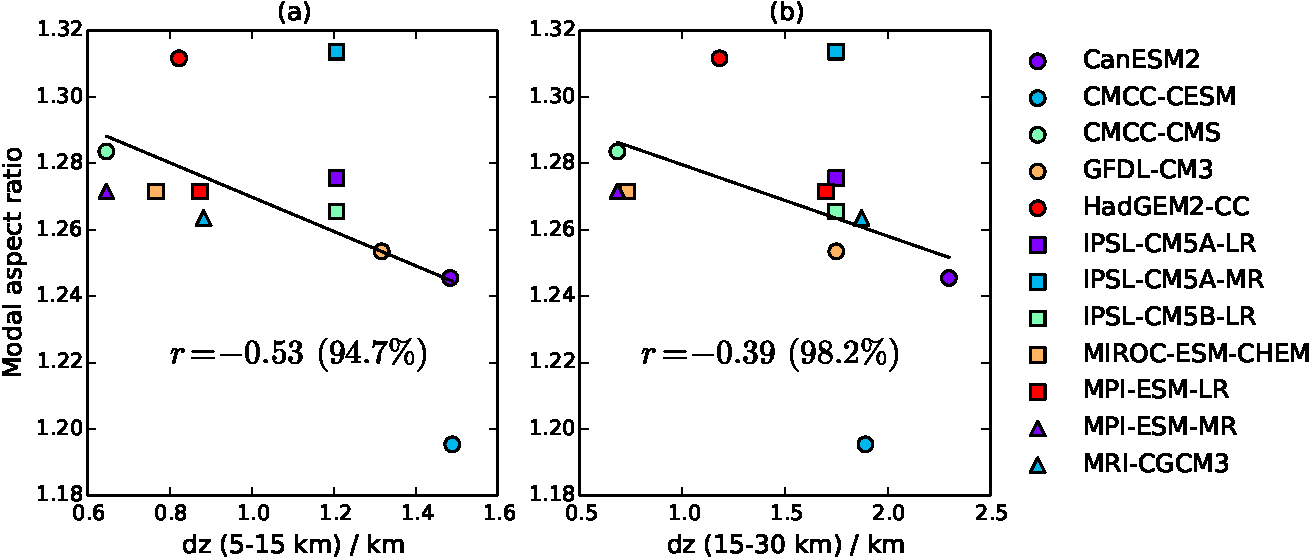
\includegraphics[width=\textwidth]{figures/chapter-models/aspect_ratio_resolution.pdf}
 \caption[Vertical resolution and modal aspect ratio.]{Expansion from Figure
   \ref{fig:scatter_matrix} of the correlation between modal aspect ratio and
   model vertical resolution over two regions (5-15~km and
   15-30~km). Correlations, $r$, are shown along with the $p$-value calculated by a
   bootstrap test with null hypothesis $r=0$.}
 \label{fig:aspect_vert_res}
\end{figure}


\subsection{Measures of stratosphere-troposphere coupling}
\label{sec:meas-strat-trop}

We have shown that zonally-averaged quantities such as polar cap $Z$ (which is
highly correlated with the NAM \citep{Kushner2010}) following split and
displaced vortex events are much less consistent among models than the NAO. This
inconsistency is dominated by differences in the North Pacific, with some models
showing positive MSLP anomalies and others negative. Interestingly, a similar
result was found in the recent study of \citet{Davini2014}, who found the
blocking pattern associated with SSWs to be consistent with that associated with
the NAM over the North Atlantic, but not over the North Pacific. 

Following \citet{Baldwin2001a}, many studies of stratosphere-troposphere
coupling have focused on the lag-height behaviour the NAM. For instance the
comparison of stratosphere-troposphere coupling in high-top and low-top CMIP5
models by \citet{Charlton-Perez2013}. This and several other studies make
further approximations as to the zonal nature of the coupling by calculating the
NAM based on zonal-mean geopotential height, according to the method of
\citet{Baldwin2009}. Our results suggest that because of the difference in model
consistency over the two ocean basins, zonal-mean diagnostics or the NAM alone
are not a good descriptors of inter-model variability. Therefore, we suggest
that the NAO index or the full two-dimensional surface fields should be shown
alongside the NAM when making inter-model comparisons.

This difference between the NAM and NAO signals in CMIP5 models may also give
some insight into the physical relevance of these two modes of variability. Some
studies have suggested that the NAO is in fact a regional manifestation of the
planetary-scale annular structure of the NAM \citep[e.g.,][]{Thompson1998,
  Wallace2002}. Furthermore, many observational studies have asserted that
tropospheric anomalies following SSWs represent the NAM
\citep[e.g.,][]{Baldwin1999,Baldwin2001a,Thompson2000}. 

On the other hand, \citet{Ambaum2001} suggested that the NAO paradigm is a more
physically relevant measure of NH variability than the NAM. They found that MSLP
anomalies over the North Atlantic and Pacific are not significantly correlated
and argued that that the annular NAM pattern is a statistical
artifact. \citet{Huth2006} also showed that principal component analysis favours
the NAO as the more physically relevant mode of variability. Furthermore,
\citet{Ambaum2002} found that changes in North Pacific tropospheric subtropical
and polar jets are much less correlated with the strength of the stratospheric
polar vortex than are the North Atlantic jets.

Under the significant assumption that the CMIP5 models can accurately represent
the physics underlying these modes of variability, our results tend to favour
the NAO rather than the NAM as the more physically relevant mode, at least in
terms of stratosphere-troposphere coupling. 


% Fluctuation-dissipation
%Discuss NAO vs NAM



\subsection{Difference between split and displaced vortex events}
\label{sec:cmip5_discuss_split_displ}

As well as the consistent NAO signal following split and displaced vortex
events, we have found that there are also some consistent differences in
anomalies following the two types of event. In particular, MSLP anomalies
following displaced vortex events are more negative over Scandinavia and Siberia
than following split vortex events. From the fact that these MSLP differences
are co-located with 100~hPa $Z$ (Figure \ref{fig:cmip5_mslp_diff}), which is in
turn related to tropopause height, it may be possible to gain some understanding
of the mechanism behind the difference in the surface response to split and
displaced vortex events. 

This co-location of surface anomalies and tropopause height is consistent with a
localised spinup/spindown caused by stretching/compression of the tropospheric
column. Changes in tropopause height are, in turn, caused by the bending of
isentropic surfaces towards PV anomalies resulting from the movement of the
stratospheric polar vortex. Such a mechanism was discussed by
\citet{Hartley1998}, \citet{Ambaum2002}, \citet{Black2002}, and in Section
\ref{sec:mechanisms}.

Other mechanisms that have been proposed for stratosphere-troposphere coupling
fail to account for these regional differences. For instance, the amplification
of intrinsic modes of variability \citep{Robinson1991} can only explain
differences which project onto these modes such as the NAO or NAM, unlike
observed difference. Stratosphere-troposphere coupling by the reflection of
planetary waves \citep{JudithPerlwitz2003,Shaw2010} also cannot explain the
observed difference since it  does not project onto the dominant tropospheric
planetary wave modes. 

This argument relates only to the mechanism underlying the \emph{difference}
between the surface responses to split and displaced vortex events, and not to
the overall responses. It is important to note that there are many similarities
in the responses, especially in the NAO region. All the mechanisms discussed in
Section ?? can be used to explain a stratospheric influence on the NAO, and
since they are not physically inconsistent with one another, it is possible that
a number may operate at the same time. 

Unfortunately, the small number of observed split and displaced vortex events
combined with large tropospheric noise means there is very little statistical
significance in the observed difference of MSLP anomalies (see Figure
\ref{fig:cmip5_mslp_diff}(a)). Hence it is not possible to compare our model and
observational results for this difference, and there remains the
possibility that CMIP5 models do not realistically represent the surface
responses to split and displaced vortex events. Therefore, it is possible that
stratosphere-troposphere coupling mechanisms in models are different to those in
the real world. 

\section{Conclusions}

Applying the method developed in Chapter \ref{cha:moments}, the climatology of
the stratospheric polar vortex and its coupling with the troposphere has been
analysed in stratosphere-resolving CMIP5 simulations. Returning to the three
main objectives of this chapter (Section \ref{sec:models_introduction}), the
following conclusions have been reached:
\begin{enumerate}

\item \textbf{How do models represent the stratospheric polar vortex and
    stratosphere-troposphere coupling?}

  A wide range of biases among CMIP5 models has been found in the average state
  of the stratospheric polar vortex. Some models have a vortex which is too
  equatorward, while others too poleward. The majority of models have a vortex
  which is too circularly symmetric. These biases have been shown to relate
  closely to biases in the frequency of split and displaced vortex events. In
  the multi-model mean, however, the frequency of these events is in agreement
  with observations. 

  Almost all models accurately simulate the more barotropic nature of split
  vortex events compared to displaced vortex events. MSLP anomalies following
  these events consistently show a negative NAO in line with observations, but
  are much less consistent in the North Pacific, leading to a large spread when
  zonal mean quantities are investigated.

\item \textbf{Is model resolution related to vortex variability?}

  There is a statistically significant correlation between near-tropopause
  vertical resolution and modal aspect ratio among models. However, this
  relationship is not seen among the two pairs of models from the same
  family. On the other hand, the tropopause region is known to be important for
  the propagation of planetary waves due to high vertical gradients of zonal
  wind shear and static stability. This may be suggestive of the need for high
  vertical resolution to accurately simulate stratospheric planetary wave
  activity and hence vortex aspect ratio. No relationships have been found
  between horizontal resolution and vortex variability.

\item \textbf{Can models be used to understand mechanisms behind
    stratosphere-troposphere coupling?}

  Consistent differences in the MSLP anomalies following split and displaced
  vortex events in the CMIP5 models have been found to be co-located with the
  difference in near-tropopause $Z$ anomalies. This is consistent with a
  localised tropospheric response to stretching or compression of the
  tropospheric column being the mechanism behind the different responses to the
  two events. It also excludes mechanisms which rely on projections onto major
  modes of variability such as the NAO or NAM. This result only applies to the
  difference between responses to split and displaced vortex events, not the
  individual responses, which share many similarities.
\end{enumerate}

% Re-address aims from introduction

%%% Local Variables:
%%% mode: latex
%%% TeX-master: "thesis"
%%% End:
